\documentclass[12pt,a4paper,accentcolor=tud1c,colorback=tud1c,colorbacksubtitle]{tudreport}

%%%%%%%%%%%%%%%%%%%%%%%%%%% Es empfiehlt sich, weitere eigene Befehle vor dem Dokument zu definieren, 
%%%%% Eigene Befehle %%%%%% da sie erst ab der Zeile ihrer Definition verwendet werden können.
%%%%%%%%%%%%%%%%%%%%%%%%%%%

\newcommand{\gf}[1]{\grqq #1\grqq}        %% Befehl \gf{Text} für "Text"

\newcommand{\name}{Elvir Sinancevic} %% Befehl \name fügt den Namen in Klammern{} ein


%%%%%%%%%%%%%%%%%%%%%%%%%%% Zu Beginn müssen alle verwendeten Pakete geladen werden.
%%%%%%%%% Pakete %%%%%%%%%% 
%%%%%%%%%%%%%%%%%%%%%%%%%%%

%%%% Layout & Struktur %%%%

\usepackage[ngerman]{babel} 	% Deutsche Trennregeln

\usepackage[T1]{fontenc}   		% für europäische Autoren ratsam; % wichtig für Trennung von Wörtern mit Umlauten

\usepackage[utf8]{inputenc} 	% Umlaute erkennen (+ ä ö ü)

\usepackage{setspace}			% Zeilenabstand fließend einstellen  
\setstretch{1.0}				% Zeilenabstand festlegen

\usepackage{geometry}			% Neue Seitenlayouts definieren

\usepackage[normalem]{ulem}		% Hilft beim Unterstreichen von Text

\usepackage{xcolor}				% Ermöglicht gefärbten Text und Boxen


%%% Grafiken % Tabellen %%%

\usepackage{graphicx}			% Grafiken einfügen und bearbeiten

\usepackage{wrapfig}			% Grafiken in fließtexte einfügen

\usepackage{multirow} 			% Tabellen mit multiplen Spalten und Zeilen

\usepackage{enumerate}			% Nummerierte Listen erstellen

\usepackage{colortbl}

%%%%%%% Mathematik %%%%%%%%%

\usepackage{amsmath} 			% Mathematik-Paket

\usepackage{tikz}				% Pfeile und Linien

\usepackage{siunitx}			% Si-einheiten per kurzeingabe

\sisetup{
	locale = DE ,				% Si-Einheiten auf Deutsch
	per-mode = symbol
}


%%%%%% Verlinkungen %%%%%%%%

\usepackage[pdftex,pdfauthor={\name},pdftitle={Arbeit von \name}]{hyperref} %Verlinkungen im Dokument, Metadaten anpassen

\usepackage{url}				% Verlinkungen auf Webseiten


%%%%%% Literatur %%%%%%%%

\usepackage{lipsum}				% Lorem Ipsum Dummy-Text

%\usepackage[backend=bibtex,style=authoryear, dashed=false]{biblatex}
\usepackage[backend=bibtex,style=numeric]{biblatex}  %% Literaturverwaltung
\bibliography{Literatur/Literatur.bib}	%% Literaturdatei aus welcher die Quellen geladen werden


%%%%%% Chemie %%%%%%%

%\usepackage[version=4]{mhchem}							% Paket für chemische Gleichungen
%\usepackage{expl3}										% Benötigt für mhchem
%\usepackage{calc}										% Benötigt für mhchem
%\RequirePackage{tikz}\usetikzlibrary{arrows.meta}		% Benötigt für mhchem (andere Pfeile)
%\usepackage{chemfig}									% Paket für chemische Figuren

%%%%%% Zusätzlich %%%%%%%
\usepackage{placeins} %Ausrichtung von Bildern

\usepackage{hyperref}  % PDA/A
\usepackage[a-1b]{pdfx}

%%%%%%%%%%%%%%%%%%%%%%% Die oben erstellten Befehle werden im Folgenden in das Titelblatt eingefügt.
%%%%% Titelblatt %%%%%% Bei abweichenden Vorstellungen können die entsprechenden Zeilen gelöscht
%%%%%%%%%%%%%%%%%%%%%%% und händisch selbst eingetragen werden


\title{Verbesserung einer existierenden Tracking-Software zur Steuerung eines Menschenmodells
	 in einer interaktiven Virtual Reality Umgebung
}  %% Titelüberschrift 

\subtitle{Improving an existing tracking software for controlling a human model in an
	 interactive virtual reality environment
} %% Untertitel

\subsubtitle{Bachelor-Thesis
			\newline
			Name: \hspace{21.3mm} \name 
			\newline 
			 Studiengang: \hspace{9.5mm} B.Sc. Informatik
			 \newline 
			 Matrikelnummer: \hspace{2.2mm} 2561916} %% Unteruntertitel

%\settitlepicture{Bilder/A9999_TelekoLogo} %% Titelbild laden

\setinstitutionlogo{Bilder/A999999_Logo}


%%%%%%%%%%%%%%%%%%%%%%% Hier beginnt das eigentliche Dokument
%%%%% Dokument   %%%%%%
%%%%%%%%%%%%%%%%%%%%%%%
% TODO: Pagenumbering
\begin{document}											% Dokumenten beginn
%--------------------------------------------------------------------------------------------------	
\maketitle		
\pagenumbering{gobble}										% Titelblat
\vspace*{\fill}
\begin{flushleft}
	\textbf{Elvir Sinancevic}
	\newline
	\textbf{Matrikelnummer: 2561916}
	\newline
	\textbf{Studiengang: Informatik B.Sc.}
	\newline\newline
	\textbf{Bachelor-Thesis}
	\newline
	\textbf{Thema: „Verbesserung einer existierenden Tracking-Software zur Steuerung eines Menschmodells in einer interaktiven Virtual Reality Umgebung"}
	\newline\newline
	Eingereicht: 27.04.2020
	\newline\newline
	Betreuer: Sebastian Günther M.Sc., Yübo Wang, M.Sc. M.A.
	\newline\newline
	Prof. Dr. Max Mühlhäuser
	\newline
	Fachgebiet Telekooperation Lab
	\newline
	Fachbereich Informatik
	\newline
	Technische Universität Darmstadt
	\newline
	Hochschulstraße 10
	\newline
	D-64289 Darmstadt
	\newline\newline
	Prof. Dr.-Ing. Reiner Anderl
	\newline
	Fachgebiet Datenverarbeitung in der Konstruktion
	\newline
	Fachbereich Maschinenbau
	\newline
	Technische Universität Darmstadt
	\newline
	Otto-Berndt-Straße 2
	\newline
	D-64287 Darmstadt	
\end{flushleft}
						% Seite mit Name, Matrikelnr, etc.
\include{Kapitel/Kapitel_Erklärung}							% Erklärung
%--------------------------------------------------------------------------------------------------
\chapter*{Kurzfassung}\label{cha:Kurzfassung}

Das Ziel dieser Forschungsarbeit ist es zu untersuchen, inwiefern Virtual Reality Technologien die Realisierung von Industrie 4.0 vorantreiben können. Aufgrund dessen wurde untersucht, welche Potenziale ein, durch die Bewegungen des Bedieners steuerbares, virtuelles menschliches Abbild (Menschmodell), in Kombination mit einer geeigneten Interaktionsschnittstelle für die virtuelle Welt, im Kontext von Industrie 4.0, liefert.
Um diese Forschungsfrage zu beantworten, wurden zunächst, nach der Untersuchung von dem aktuellen Stand der Technik der Industrie, der industriellen Fertigung und der Virtual Reality, in einer Konzeptionsphase Anforderungen aufgestellt, die daraufhin bei der Implementierung eines Anwendungsbeispiels berücksichtigt wurden. Für die Implementierung wurde die Entwicklungsumgebung Unity Engine verwendet. Daraufhin wurden die aufgestellten Anforderungen anhand der fertigen Implementierung validiert.
Das entstandene Anwendungsbeispiel ist in der Lage, die Potenziale eines solchen Menschmodells in der Industrie aufzuzeigen. Durch das Menschmodell könnte beispielsweise die standortunabhängige Begehung und Steuerung von Produktionsanlagen, über einen entsprechenden virtuellen Klon der Anlage, möglich gemacht werden.
Aufgrund dessen lässt sich deutlich sagen, dass Virtual Reality Technologien im Kontext von Industrie 4.0 berücksichtigt werden sollten. Dennoch Bedarf es noch an viel Forschung und Entwicklung in diesem Bereich, da die Wandlung zu Industrie 4.0 einen interdisziplinären Entwicklungsprozess darstellt, der die klassischen Ausmaße des Maschinenbaus übersteigt und daher eine engere Zusammenarbeit zwischen Maschinenbauern und Informatikern erfordert.
\newline
\textbf{Schlüsselwörter:} Industrie 4.0, virtuelle Realität, Menschmodell, Interaktion, Unity Engine

%--------------------------------------------------------------------------------------------------
\begingroup
\let\clearpage\relax
\chapter*{Abstract}\label{sec:Abstract}
The goal of this research project is to investigate the extent to which virtual reality technologies can drive the realization of Industry 4.0. Based on this, the potential of a virtual human image (human model), which can be controlled by the movements of the operator, in combination with a suitable interaction interface for the virtual world, in the context of Industry 4. 0, was investigated.
In order to answer this research question, first of all, after examining the current state of the art in industry, industrial production and virtual reality, requirements were established in a conception phase, which were then taken into account when implementing an application example. The Unity Engine development environment was used for the implementation. Thereupon, the established requirements were validated against the finished implementation.
The resulting application example is able to demonstrate the potential of such a human model in an industrial setting. The human model could, for example, make it possible to inspect and control production plants from any location using a corresponding virtual clone of the plant.
Based on this, it can be clearly stated that virtual reality technologies should be considered in the context of Industry 4.0. Nevertheless, there is still a need for much research and development in this area, since the transformation to Industry 4. 0 represents an interdisciplinary development process that exceeds the classic dimensions of mechanical engineering and therefore requires closer cooperation between mechanical engineers and computer scientists.
\newline
\textbf{Keywords:} Industry 4.0, Virtual Reality, human model, interaction, Unity Engine

\endgroup							% Abstract
%--------------------------------------------------------------------------------------------------	
\cleardoublepage											% Cleardoublepage
\pagenumbering{roman}										% Römische Nummerierung
\phantomsection												% Phantomsection
\addcontentsline{toc}{chapter}{Inhaltsverzeichnis}			% Verlinkung im Inhaltsverzeichnis
\tableofcontents											% Inhaltsverzeichnis
\cleardoublepage											% Cleardoublepage
%--------------------------------------------------------------------------------------------------
\phantomsection												% Phantomsection
\addcontentsline{toc}{chapter}{Abbildungsverzeichnis}		% Verlinkung im Inhaltsverzeichnis
\listoffigures												% Abbildungsverzeichnis
\cleardoublepage											% Cleardoublepage
%--------------------------------------------------------------------------------------------------	
\phantomsection												% Phantomsection
\addcontentsline{toc}{chapter}{Abkürzungen}					% Abkürzungen
\include{Kapitel/Kapitel_Abkürzungen}						% Verlinkung im Inhaltsverzeichnis
\cleardoublepage											% Cleardoublepage
%--------------------------------------------------------------------------------------------------
\pagenumbering{arabic}										% Arabische Nummerierung
%--------------------------------------------------------------------------------------------------
\chapter{Einleitung} \label{cha:Einleitung}	

Kaum einem Begriff wird in der Industrie momentan mehr Bedeutung geschenkt als Industrie 4.0, welcher erstmalig auf der Hannover Messe 2011 auftauchte und seit Jahren Bestandteil der High-Tech-Strategie der Bundesregierung ist \cite{8}. Der Begriff Industrie 4.0 „steht für die 4. Industrielle Revolution, einer neuen Stufe der Organisation und Steuerung der gesamten Wertschöpfungskette" \cite{1} , und ist das Ergebnis der industriellen Revolutionen der vergangenen 260 Jahre. Durch das Internet der Dinge und Dienstleistungen und die zunehmende Digitalisierung der Industrie, führt dies langfristig zu einer stärkeren Vernetzung von „Menschen, Maschinen und Werkstücken durch modernste Informations- und Kommunikationstechnik" \cite{6}, also auch durch Virtual Reality Technologien. Grundlage dabei bilden Cyper-Physische-Systeme, „die bezogen auf moderne Steuerungssysteme, eingebettete Softwaresysteme und eine Internetadresse besitzen" \cite{1} um die realen mit virtuellen Produktionsprozessen zu verknüpfen \cite{11}.
\newline
Im Hinblick auf die zunehmende Digitalisierung und auf die Cyber-Physischen-Systeme, wird im Folgenden wird die Frage behandelt, wie durch das Einsetzen von Virtual Reality, konkreter noch durch das Einsetzen von einem Menschmodell (steuerbares, virtuelles Abbild eines Menschen) in einer interaktiven Virtual Reality Umgebung, die Realisierung von Industrie 4.0 vorangetrieben werden kann.

%--------------------------------------------------------------------------------------------------
\section{Motivation}\label{sec:Motivation}
Diese Arbeit legt einen Fokus auf Mensch-Maschine Interaktion in der virtuellen Welt. Auf Basis der bei einem Bachelorpraktikum am Fachgebiet Datenverarbeitung in der Konstruktion (DiK) im Wintersemester 2018/2019 gewonnenen Kenntnisse über ein Menschmodell in einer Virtual Reality Umgebung, soll das ursprüngliche Menschmodell verbessert und um eine Interaktionsschnittstelle erweitert werden.
\newline
Virtual Reality Technologien, also „die Darstellung und Wahrnehmung der Wirklichkeit und ihrer physikalischen Eigenschaften in einer digitalen, interaktiven Umgebung in Echtzeit" \cite[S.1]{4} finden in der heutigen Zeit „eine immense Anwendungsbreite in allen Lebensbereichen" \cite[S.1]{4}, vor allem auch in der Industrie. Langfristig sollen „Mensch, Maschinen, Anlagen, Logistik und Produkte [...] in der Industrie 4.0 direkt miteinander kommunizieren" \cite[S.2]{4}.
\newline
Aufgrund dessen kann durch ein Menschmodell in einer interaktiven virtuellen Umgebung das Potenzial von Virtual Reality Technologien im Kontext von Industrie 4.0, mit Hilfe eines geeigneten Anwendungsbeispiels, dargestellt werden.

%--------------------------------------------------------------------------------------------------
\section{Zielsetzung}\label{sec:Zielsetzung}
Das Ziel dieser Arbeit liegt in der Erschaffung eines Prototypen eines Menschmodells und einer Interaktionsschnittstelle, um dem Bediener das Interagieren mit einer virtuellen Umgebung zu ermöglichen, welche beispielsweise eine Produktionsanlage repräsentiert. Weiterhin soll das entstandene Anwendungsbeispiel das Potenzial von Virtual Reality Technologien im Kontext von Industrie 4.0 darstellen.
\newpage

%--------------------------------------------------------------------------------------------------
\section{Aufbau der Arbeit}\label{sec:AufbauDerArbeit}
Der Aufbau dieser Arbeit ist in Abbildung \ref{fig:AufbauDerArbeit} dargestellt.
\begin{figure}[h]
	\centering
	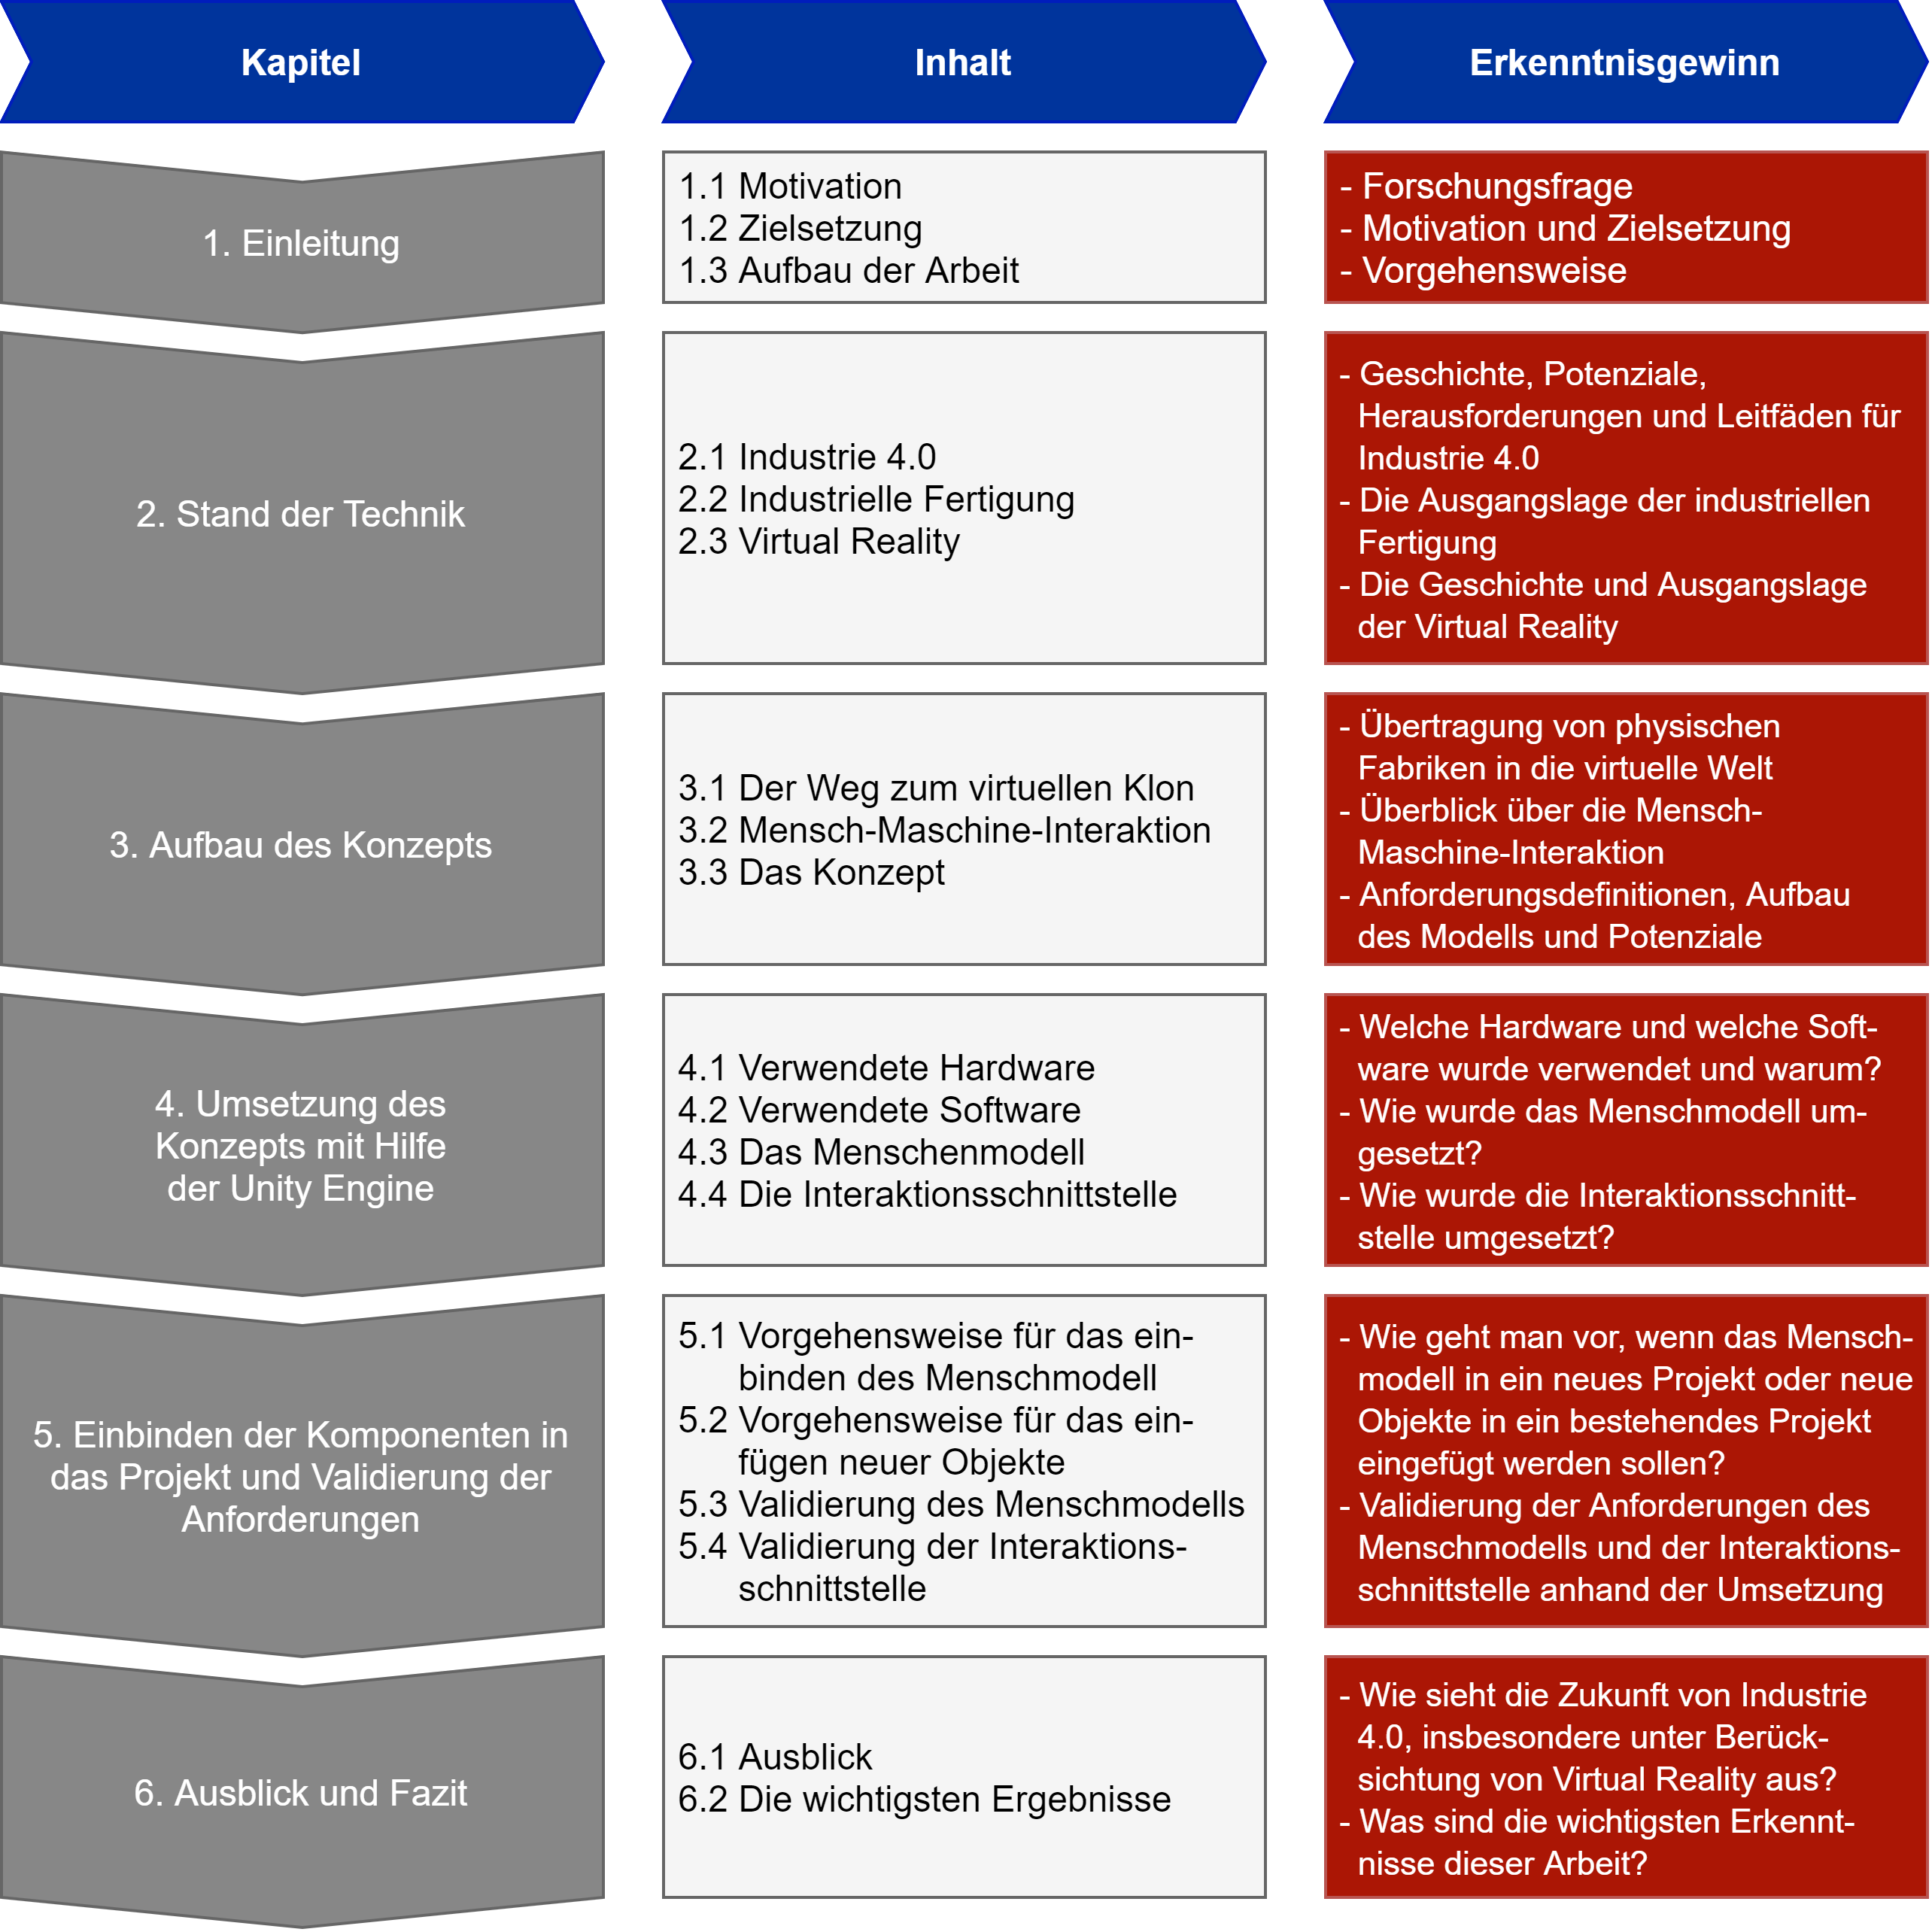
\includegraphics[width=1\linewidth]{Bilder/A55_AufbauNeu}
	\caption{Der Aufbau der Arbeit, eigene Abbildung}
	\label{fig:AufbauDerArbeit}
\end{figure}
\newline\newline
Zunächst wird, nach der Einleitung, in Kapitel \ref{cha:StandDerTechnik} der aktuelle Stand der Technik thematisiert. Aufgrund dessen gibt es in Unterkapitel \ref{sec:Industrie4.0} einen Einblick in die Geschichte der industriellen Revolutionen und der Wandlungen im Bereich der Informations- und Kommunikationstechnik (Kapitel \ref{sec:GeschichteIndustrie4}), bevor anschließend die Potenziale (Kapitel \ref{sec:PotentialeIndustrie4.0}) und Herausforderungen (Kapitel \ref{sec:HerausforderungenUmsetzung}) von Industrie 4.0 erläutert werden. Daraufhin werden noch zwei Leitfäden, die Unternehmen bei dem Wandel zu Industrie 4.0 unterstützten sollen (Kapitel \ref{sec:LeitfadenUmsetung}), erläutert. Anschließend gibt es in Unterkapitel \ref{sec:IndustrielleFertigung} noch eine Einführung in die Ausgangslage der industriellen Fertigung, insbesondere werden dabei der Produktlebenszyklus (Kapitel \ref{sec:Produktlebenszyklus}), die Automatisierungspyramide (Kapitel \ref{sec:Automatisierungspyramide}) und der Wandel der Automatisierungspyramide im Kontext von Industrie 4.0 (Kapitel \ref{sec:AutomatisierungspyramideUndIndustrie4.0}) erläutert. Zum Abschluss gibt es in Unterkapitel \ref{sec:VR} noch eine Einführung in das Thema virtuelle Realität, insbesondere in die Geschichte (Kapitel \ref{sec:VRGeschichte}) und die Potenziale (Kapitel \ref{sec:VRPotentialUndAusblick}) von Virtual Reality Technologien.
\newline
Im darauf folgenden Kapitel \ref{cha:AufbauDesKonzepts} wird das Konzept erläutert. Aufgrund dessen wird in Unterkapitel \ref{sec:PhysischZumKlon} zunächst der Prozess von der physischen Produktionsanlage bis hin zu ihrem virtuellen Klon erläutert und die Arbeit in diesem Prozess eingeordnet. Daraufhin gibt es in Unterkapitel \ref{sec:MMInteraktion} einen Überblick über die Mensch-Maschine-Interaktion im Kontext dieser Arbeit, bevor die Arbeit auch in diesem Kapitel entsprechend eingeordnet wird. Anschließend wird in Unterkapitel \ref{sec:ModellAufbau} das eigentliche Konzepts des Menschmodells aufgebaut, indem zunächst die Anforderungen an das Menschmodell und die Interaktionsschnittstelle erläutert werden (Kapitel \ref{sec:AnforderungenKonzept}). Des Weiteren gibt es eine Einführung in das Functional-Mockup Interface (Kapitel \ref{sec:DasFMU}), bevor erläutert wird, wie die Umsetzung des Menschmodells mit Hilfe des FMI Standards auszusehen hätte (Kapitel \ref{sec:ModelAufbau}) und worin die Potenziale liegen würden (Kapitel \ref{sec:PotenzialeFMU}).
\newline
Aufbauend auf dem im vorherigen Kapitel gewonnen Verständnis und insbesondere unter Berücksichtigungen der gestellten Anforderung an das Menschmodell und die Interaktionsschnittstelle, wird in Unterkapitel \ref{cha:Umsetzung} die Umsetzung des Konzepts mit Hilfe der Unity Engine erläutert. Aufgrund dessen gibt es in Kapitel \ref{sec:Hardware} zunächst eine Einführung in die verwendete Hardware. Dazu gehören die Brille und ihr Zubehör (Kapitel \ref{sec:GrundHardware}), die Tracker (Kapitel \ref{sec:TrackerVive}) und auch die Befestigungen für die Tracker (Kapitel \ref{sec:TrackerBefestigung}). Daraufhin wird in Unterkapitel \ref{sec:Software} die verwendete Software, also die VIVE Wireless Anwendung (Kapitel \ref{sec:VIVEWireless}), die SteamVR Anwendung (Kapitel \ref{sec:SteamVR}) und die Entwicklungsumgebung Unity Engine mit den genutzten Plugins (Kapitel \ref{sec:UnitEngine}), erläutert. Anschließend wird in Unterkapitel \ref{sec:DasMenschmodell} die Umsetzung des Menschmodells erklärt, vom Grundgerüst des Menschmodells (Kapitel \ref{sec:MMModell}), über die ergänzenden Komponenten (Kapitel \ref{sec:MMKomponenten}) und erstellten Skripte (Kapitel \ref{sec:MMCode}), bis hin zu einer kurzen Zusammenfassung des entstandenen Modells (Kapitel \ref{sec:MMFunktionen}). Schließlich wird in Unterkapitel \ref{sec:DieInteraktionsschnittstelle} die Umsetzung der Interaktionsschnittstelle erläutert. Daher werden zunächst das Grundgerüst (Kapitel \ref{sec:GrundgerüstInteraktion}), daraufhin die ergänzenden Komponenten (Kapitel \ref{sec:WeitereTeileInteraktion}) und anschließend eine kurze Zusammenfassung der entstandenen Interaktionsschnittstelle (Kapitel \ref{sec:ZusammenfassungInteraktion}) vorgestellt.
\newline
In Kapitel \ref{cha:ValidierungDesKonzepts} gibt es zunächst im Unterkapitel \ref{sec:MenschmodellEinbinden} eine Einführung in die Vorgehensweise beim Einbinden des Menschmodells und der Interaktionsschnittstelle in ein neues Projekt, bevor anschließend in Unterkapitel \ref{sec:ObjekteEinbinden} die Vorgehensweise beim Einfügen neuer Objekte in der Umgebung erläutert wird. Schließlich werden in den Unterkapiteln \ref{sec:ValidMensch} und \ref{sec:ValidInteraktion} die gestellten Anforderungen an das Menschmodell und die Interaktionsschnittstelle, unter Berücksichtigung der erläuterten Umsetzung des Konzepts mit Hilfe der Unity Engine, validiert.
\newline
Abschließend gibt es in Kapitel \ref{cha:AusblickUndFazit} in Unterkapitel \ref{sec:Ausblick} einen Ausblick, der sich damit befasst, wie die Zukunft von Industrie 4.0, insbesondere im Hinblick auf Virtual Reality, aussehen könnte, bevor in Unterkapitel \ref{sec:ZusammenfassungErgebnisse} die wichtigsten Erkenntnisse der Arbeit zusammengefasst werden.

%--------------------------------------------------------------------------------------------------						% Einleitung
%--------------------------------------------------------------------------------------------------	
%--------------------------------------------------------------------------------------------------
\chapter{Stand der Technik}\label{cha:StandDerTechnik}

\lipsum[2]

%--------------------------------------------------------------------------------------------------
\section{Industrie 4.0}\label{sec:Industrie4.0}
Der Begriff Industrie 4.0 „steht für die 4. Industrielle Revolution, einer neuen Stufe der Organisation und Steuerung der gesamten Wertschöpfungskette über den Lebenszyklus von Produkten“ [1, Anderl, Vortrag 2015]. Dies führt zum einem zu einer zunehmenden Vernetzung von „Mensch, Maschinen und Werkstücken durch Modernste Informations- und Kommunikationstechnik“ [6, BDI, Was ist Industrie 4.0], zum anderen auch zu einer zunehmenden „Vernetzung der realen mit der virtuellen Welt“ [7, DIN, Def. Ind.4].
\newline
Grundlage dieser Wandlung in der Industrie sind sogenannte Cyber-Physische-Systeme (CPS), also moderne Steuerungssysteme mit eingebetteten Softwaresystemen und Anbindung an das Internet [1, Anderl, Vortrag 2015], was eine zunehmende Verschmelzung von Fertigungsprozessen und Informationstechnologie zur Folge hat [7, DIN, Def. Ind.4].
\newline

\lipsum[2]

\subsection{Die Geschichte industrielle Revolution}\label{sec:IndustrielleRevolution}

\lipsum[2]

\subsection{Potentiale von Industrie 4.0}\label{sec:PotentialeIndustrie4.0}

\lipsum[2]

\subsection{Herausforderungen bei der Umsetzung}\label{sec:HerausforderungenUmsetzung}

\lipsum[2]

\subsection{Leitfaden für Industrie 4.0}\label{sec:LeitfadenUmsetung}

\lipsum[2]

%--------------------------------------------------------------------------------------------------
\section{Mensch-Computer Interaktion}\label{sec:HCI}

\lipsum[2]

\subsection{Die Geschichte der Mensch-Computer Interaktion}\label{sec:HCIGeschichte}

\lipsum[2]

\subsection{Relevanz für meine Arbeit}\label{sec:RelevanzHCI}

\lipsum[2]

\subsection{???}\label{sec:???}

\lipsum[2]

%--------------------------------------------------------------------------------------------------
\section{Virtual Reality}\label{sec:VR}

\lipsum[2]

\subsection{Die Geschichte von Virtual Reality Hardware}\label{sec:VRGeschichte}

\lipsum[2]

\subsection{Stand der Technik}\label{sec:VRStandDerTechnik}

\lipsum[2]

\subsection{Technische Herausforderungen}\label{sec:VRHerausforderungen}
\lipsum[2]

\subsection{Potential und Ausblick}\label{sec:VRPotentialUndAusblick}

\lipsum[2]

\subsection{????}\label{sec:????}

\lipsum[2]

%--------------------------------------------------------------------------------------------------					% Stand der Technik
%--------------------------------------------------------------------------------------------------	
%--------------------------------------------------------------------------------------------------
\chapter{Aufbau des Konzepts}\label{cha:AufbauDesKonzepts}

In diesem Kapitel wird der Aufbau des Konzepts erklärt. Daher gibt es zu erst einen Einblick in den Digitalisierungsprozess von Produktionseinlagen. Daraufhin wird diese Arbeit in das Gesamtkonzept der Mensch-Maschine Interaktion eingeordnet. Schließlich wird der Aufbau des Modells mithilfe des Functional-Mockup Interfaces erklärt.

%--------------------------------------------------------------------------------------------------
\section{Von der physischen Produktionsanlage zum virtuellen Klon}\label{sec:PhysischZumKlon}

Um die Produktionsabläufe einer Fabrik in einer virtuellen Welt abzubilden gibt es insgesamt sieben Schritte die befolgt werden müssen.

\begin{enumerate}
	\item \textbf{Scannen der Fabrik} \\
	Im ersten Schritt werden die Produktionsräume inklusive der Produktionsanlagen gescannt. Das Ergebnis dieses Scans ist eine Punktwolke.
	\item \textbf{Umwandlung des Scans} \\
	Der Scan muss von einer Punktewolke in CAD Modelle umgewandelt werden. Da die CAD Modelle zu groß und daher unpraktikabel für die Entwicklungsumgebung Unity sind, werden diese in das OBJ Format umgewandelt. Die Modelle sind für den späteren Aufbau des virtuellen Klons der echten Produktionsanlage notwendig.
	\item \textbf{Abbildung: Produktionsanlage $\rightarrow$ Modell} \\
	Es wird ein physisches Modell zur Darstellung einiger wichtiger Herausforderungen der echten Produktionsanlage gebaut. Dies könnte Beispielsweise die Form einer Produktionsstraße mit mehreren Stationen besitzen.
	\item \textbf{Virtueller Aufbau} \\
	Das physische Modell der echten Produktionsanlage aus Schritt drei wird in der virtuellen Welt abgebildet (virtueller Klon) und mit dem Menschmodell begehbar gemacht. Dieser Schritt erlaubt die virtuelle Planung einer Produktionsanlage.
	\item \textbf{Konnektivität und Kommunikation} \\
	Die Produktionsanlagen des physischen Modells werden mit der Cloud vernetzt um eine bidirektionale Kommunikation zwischen dem physischem Modell und dem virtuellen Klon zu ermöglichen.
	\item \textbf{Interaktion} \\
	Die Interaktion mit zwischen dem Bediener und den Produktionsanlagen in der virtuellen Welt wird implementiert. Es müssen unter Umständen anwendungsspezifische Benutzeroberflächen implementiert werden.
	\item \textbf{Skalierung} \\
	Skalierung der Vorgehensweise durch Anwendung von Schritt vier bis sechs auf die echte Produktionsanlage.
\end{enumerate}
Durch das Einhalten dieser Schritte erhält man einen virtuellen Klon der echten Produktionsanlage. Diesen virtuellen Klon kann man für viele Zwecke einsetzen, dazu gehören Beispielsweise die Produktionsplanung oder das Fernsteuern von Produktionsanlagen. Das Ergebnis dieser Arbeit kommt bei Schritt vier und sechs zum Einsatz [Quelle Yübo?].

%--------------------------------------------------------------------------------------------------
\section{Mensch-Maschine Interaktion im Kontext dieser Arbeit}\label{sec:MMInteraktion}
\begin{figure}[h]
	\centering
	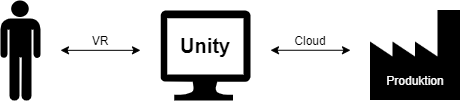
\includegraphics[width=0.7\linewidth]{Bilder/A19_MMI}
	\caption{Mensch-Maschine Interaktion im Kontext dieser Arbeit, eigene Abbildung}
	\label{fig:MMI}
\end{figure}
\noindent Durch die Abbildung der echten Produktionsanlage in der virtuellen Welt findet die Mensch-Maschine-Interaktion in zwei Schritten statt. Im ersten Schritt interagiert der Mensch mit der Software (dem Computer) über VR-Hardware. Dieser Computer interagiert dann über eine Cloud mit der echten Produktionsanlage. Die Kommunikation findet in beiden Schritten bidirektional statt.
\newline\newline
Diese Arbeit befasst sich mit dem ersten Schritt der oben erklärten Mensch-Maschine Interaktion. Für dem Rest dieser Arbeit werden wir annehmen, dass es bereits eine geeignete Infrastruktur für die Kommunikation zwischen dem Computer und der Produktionsanlage über eine Cloud gibt.

%--------------------------------------------------------------------------------------------------
\section{Das Modell der Interaktivität mit einem Menschmodell}\label{sec:ModellAufbau}
Basierend auf den im folgenden definierten Anforderungen soll mit Hilfe des Functional-Mockup Interfaces ein Modell aufgebaut werden.

\subsection{Anforderungen an das Modell}\label{sec:AnforderungenModell}
Da das Modell aus zwei Teilen besteht, haben beide Teile Ihre eigenen Anforderungen. Diese werden im Folgenden erläutert. Das Ziel ist es ein Menschmodell zu schaffen, welches interaktiv mit seiner Umgebung interagieren kann.

\subsubsection{Menschmodell}
\begin{enumerate}
	\item \textbf{Genauigkeit} \\
	Die Genauigkeit der Abbildung der Tracking-Daten auf das virtuelle menschliche Abbild ist von zentraler Bedeutung. Vor allem in einem Szenario, bei dem sich mehrere virtuelle menschliche Abbildungen in einem virtuellen Klon einer Produktionsanlage aufhalten ist die möglichst genaue Abbildung unabdingbar, um Beispielsweise auf andere Bediener in der virtuellen Welt Rücksicht nehmen zu können.
	\item \textbf{Echtzeit} \\
	Sowohl das Tracking des Bedieners als auch die Abbildung der Tracking-Daten auf das virtuelle menschliche Abbild sind echtzeitkritische Anwendungen. Die Verzögerungen müssen möglichst gering sein um eine gute Nutzbarkeit zu ermöglichen.
	\item \textbf{Interoperabilität} \\
	Das Menschmodell muss umgebungsunabhängig implementiert werden. Die bedeutet, dass das Menschmodell in beliebigen Umgebungen (Fabriken, Produktionshallen, etc.) eingesetzt werden kann.
	\item \textbf{Modularität} \\
	Sowohl einzelne Komponenten als auch das ganze Menschmodell an sich unterliegen der Anforderung der Modularität, um in Zukunft Verbesserungen oder Erweiterungen am Modell durchführen zu können.
\end{enumerate}

\subsubsection{Interaktion}
\begin{enumerate}
	\item \textbf{Bidirektionalität} \\
	Der Informationsaustausch muss bidirektional stattfinden. Das bedeutet, dass der Bediener über geeignete, leicht zu verstehende, optisch ansprechende und vor allem einheitliche Benutzeroberflächen interagieren kann. Einerseits ermöglichen diese Benutzeroberflächen dem Bediener das Interagieren mit Produktionsanlagen, andererseits werden auf diesen Benutzeroberflächen für den Bediener relevante Informationen in geeigneter Form dargestellt.
	\item \textbf{Genauigkeit} \\
	Auch bei der Interaktion spielt die Genauigkeit eine wichtige Rolle. Der Bediener sollte intuitiv, mit relativ geringen Lernaufwand, schnell und vor allem präzise mit der Umgebung interagieren können.
	\item \textbf{Echtzeit} \\
	Die Interaktion muss mit einer möglichst geringen Verzögerung stattfinden, um dem Nutzer schnelle Reaktionen und spontane Anpassungen oder Verbesserungen zu ermöglichen.
	\item \textbf{Interoperabilität} \\
	Die Interaktion muss über eine einheitliche Schnittstelle stattfinden um Interoperabilität zu gewährleisten, sodass sich die Funktionalität auf beliebige Maschinen und Produktionsanlagen übertragen lässt.
	\item \textbf{Modularität} \\
	Durch das Gewährleisten der Modularität wird sichergestellt, dass die Interaktion in Zukunft auch auf neue VR-Hardware übertragen werden kann ohne das die gesamte Software neu geschrieben werden muss.b
\end{enumerate}
Durch das Einhalten dieser Herausforderungen ergibt sich ein Menschmodell, welches in Echtzeit die Bewegungen des Bedieners auf das virtuelle Menschliche Abbild projiziert. Des Weiteren ermöglicht das Modell dem Bediener in der virtuellen Welt mit dem virtuellen Klon der Produktionsanlage zu interagieren. Da von Anfang an ein Fokus auf Interoperabilität und Modularität gelegt wird, ist das ganze Modell erweiterbar und an verschiedene Hardware und unterschiedliche Einsatzzwecke anpassbar.

\subsection{Das Functional-Mockup Interface}\label{sec:DasFMU}
Das Functional-Mockup Interface (FMI) ist ein ursprünglich von der Daimler AG entwickelter unabhängiger Standard für den Austausch von dynamischen Modellen und Co-Simulation. Zum Einsatz kommt das Functional-Mockup Interface beispielsweise beim Modellaustausch oder der Co-Simulation zwischen Zulieferern und den OEMs (Original Equipment Manufacturer) [24, FMI-Paper, S.1].
Anfang 2010 wurde die erste Version (Version 1.0) des FMI Standards veröffentlicht, welche zunächst nur den Modellaustausch unterstützte. Einige Monate später folgte dann die Unterstützung für Co-Simulation. Mittlerweile gab weitere Nachfolger Versionen. Die aktuellste Version (Version 2.0.1) wurde im Oktober 2019 veröffentlicht, unterscheidet sich aber von der Vorgängerversion (Version 2.0) aus dem Jahr 2014 nur durch einige Bugfixes [2, FMI-Spez, S.2].
Da es neben den anwendungsspezifischen Standards (z.B. Matlab/Simulink: S-Functions) zunächst keinen unabhängigen Standard für den Austausch von Modellen oder die Co-Simulation gab [24, FMI-Paper, S.1], liegt der größte Vorteil des FMI-Standards in seiner Unabhängigkeit.
\newline\newline
Wie bereits erwähnt gibt es für den FMI Standard zwei übergeordnete Anwendungsszenarien:
\begin{enumerate}
	\item \textbf{Modellaustausch} \\
	Der FMI Standard ermöglicht Modellierungsumgebungen ein dynamisches System Modell in C-Code zu repräsentieren, sodass dieses Modell auch in anderen Modellierungsumgebungen genutzt werden kann. Ermöglicht wird dies durch die Darstellung der Modelle mit Hilfe von mathematischen Gleichungen (z.B. Algebraische Gleichungen, Differentialgleichungen oder Diskrete Gleichungen), welche auch Zeit-, Zustands- oder Schritt-Events enthalten können. Es werden große Modelle und sowohl die offline als auch die online Simulation unterstützt [25, FMI-Spez, S.4].
	\item \textbf{Co-Simulation} \\
	Des Weiteren ermöglicht der FMI Standard das Verbinden von mehreren Subsystem, welche über vordefinierte Kommunikationsschnittstellen kommunizieren und somit eine Co-Simulationsumgebung schaffen. Dabei wird der Datenaustausch und die Synchronisation zwischen den einzelnen Subsystemen durch einen sogenannten Master Algorithmus gesteuert. Bei den Master Algorithmen ist zu beachten, dass diese kein Teil des eigentlichen FMI Standards sind [25, FMI-Spez, S.4]. Daher sind die Master Algorithmen nicht standardisiert und können unterschiedliche zusätzliche Funktionalitäten wie z.B. den Austausch von Variablen unterstützen [24, FMI-Paper, S.1].
\end{enumerate}
Die grundlegenden Komponenten die beim Einsatz des FMI Standards immer zum Einsatz kommen sind das „FMI Application Programming Interface (C)“ und das „FMI Description Schema (XML)“. Ersteres enthält dabei alle benötigten Gleichungen des Models. Dabei kommt die Programmiersprache C zum Einsatz, da sie portabel ist und auch für den Einsatz in eingebetteten System geeignet ist. Die XML-Datei (vgl. Abbildung \ref{fig:FMIOverview}) hingegen enthält die Definitionen aller Variablen in einem standardisierten Format. Diese Variablendefinition ist durchaus eine komplexe Datenstruktur. Die Simulationstools können selber entscheiden wie sie mit diesen Daten umgehen und wie sie die Daten in ihren Programmen repräsentieren möchten. Dieser Ansatz erlaubt das Speichern und Laden der Variablendefinitionen ohne Einbußen bei der Performance in der Programmiersprache der Simulationsumgebung, wie z.B. C\# oder Java [25, FMI-Spez, S8].
\newline
\begin{figure}[h]
	\centering
	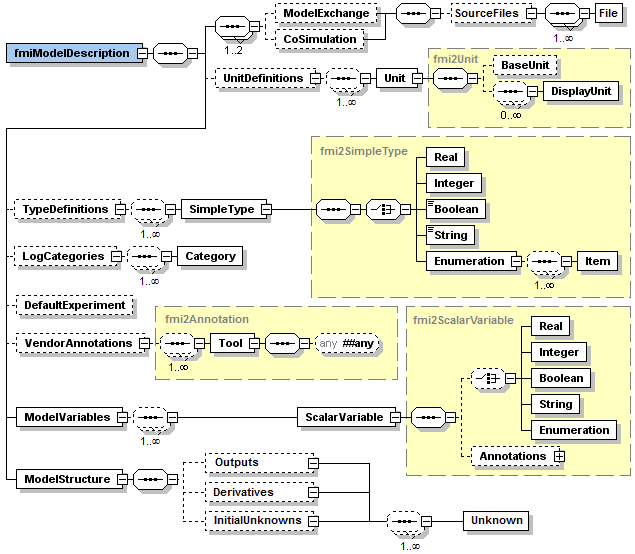
\includegraphics[width=0.7\linewidth]{Bilder/A20_FMIOverview}
	\caption{Aufbau der FMI Variablenbeschreibung [25, FMI-Spez, S.30]}
	\label{fig:FMIOverview}
\end{figure}
\newline
hi

\begin{figure}[h]
	\centering
	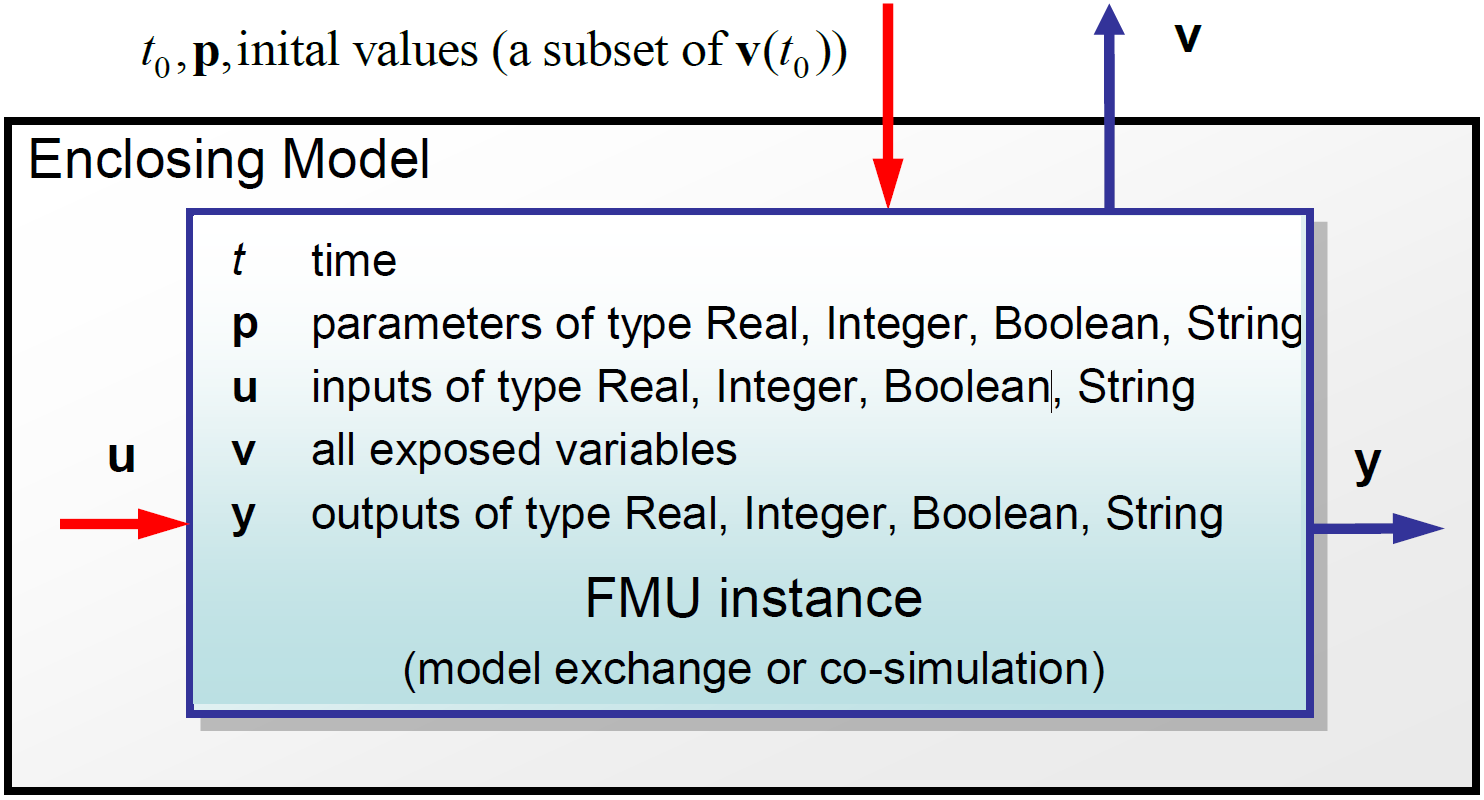
\includegraphics[width=0.7\linewidth]{Bilder/A21_FMIBlock}
	\caption{FMU Instanz [25, FMI-Spez, S.9]}
	\label{fig:FMIBlock}
\end{figure}

\begin{figure}[h]
	\centering
	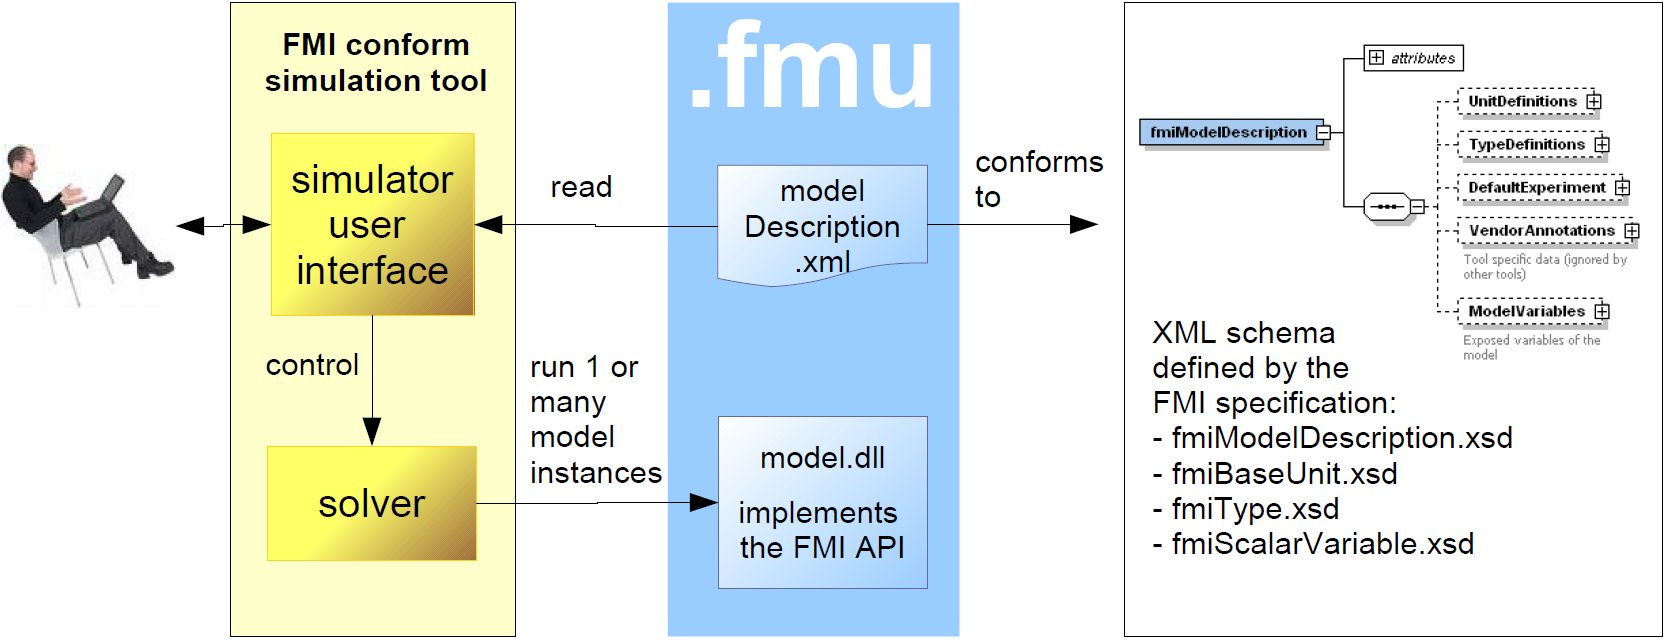
\includegraphics[width=1\linewidth]{Bilder/A22_User-FMU-FMI}
	\caption{Einordnung der FMU in dem Environment (?) [26, QTronic, S.7]}
	\label{fig:FMUEinordnung}
\end{figure}


\subsection{Der Aufbau des Models}\label{sec:ModelAufbau}
%--------------------------------------------------------------------------------------------------						% Konzept
%--------------------------------------------------------------------------------------------------	
%--------------------------------------------------------------------------------------------------
\chapter{Umsetzung des Konzepts mit Hilfe der Unity Enginge}\label{cha:Umsetzung}
In diesem Kapitel wird die Umsetzung des Menschmodells und der Interaktion in der Entwicklungsumgebung der Unity Engine vorgestellt. Daher gibt es zunächst einen Einblick in die genutzte Hardware und Software, bevor das Menschmodell und die Interaktionsschnittstelle genauer erläutert werden.
%--------------------------------------------------------------------------------------------------
\section{Eingesetzte Hardware}\label{sec:Hardware}
Für die Umsetzung dieses Projektes wurde die Virtual Reality Brille \textbf{VIVE Pro} (Vgl. Abbildung \ref{fig:ViveproKit}) vom Hersteller HTC verwendet, da sie eine der Leistungsstärksten Brillen auf dem Markt ist. Zu den Stärken dieser Brille gehören das kontrastreiche OLED-Display, die sehr hohe Auflösung von 1440 x 1600 Pixeln pro Auge, eine Bildwiederholrate von 90Hz, ein Sichtfeld von 110 Grad und vor allem die Möglichkeit die Brille mit Hilfe des \textbf{Vive Wireless Sets} (Vgl. Abbildung \ref{fig:WirelessKit}) kabellos zu verwenden. Es ist anzumerken, dass für das kabellose Verwenden dieser VR Brille eine \textbf{Erweiterungskarte} in den PC eingebaut werden muss um einen speziellen \textbf{Empfänger} für die Signale der Brille anzuschließen. Des Weiteren muss ein \textbf{Sender} an der VR-Brille angebracht werden, welcher mit dem am PC angeschlossenen Empfänger kommuniziert und durch einen \textbf{mobilen Akku} mit Strom versorgt wird. Der mitgelieferte mobile Akku ermöglicht einen kabellosen Einsatz der VR Brille für bis zu sechs Stunden (Vgl. Abbildung \ref{fig:WirelessKit}) [28, ViveWeb].
\newline\newline
Um die Brille zu verwenden bedarf es mindesten zwei der sogenannten \textbf{SteamVR 2.0 Basisstationen} (Vgl. Abbildung \ref{fig:ViveproKit}), welche dem Bediener in Kombination mit des Vive Wireless Adapters eine enorme Bewegungsfreiheit ermöglichen. Beim Einsatz von zwei solcher Basisstationen ist eine Raumgröße von bis zu 5m x 5m, also 25m² möglich. Es ist sogar möglich bis zu vier solcher Basisstationen zu Verwenden und somit eine Raumgröße von bis zu 10m x 10m, also 100m² zu unterstützen [28, ViveWeb].
\newline\newline
Ein weiteres notwendiges Zubehör der Brille sind die beiden \textbf{Controller} (Vgl. Abbildung \ref{fig:ViveproKit}), die es dem Bediener ermöglichen mit der virtuellen Umgebung zu interagieren. Beide Controller werden wie die VR Brille durch die Basisstationen im Raum geortet und liefern Informationen über ihre eigene Position und Ausrichtung im Raum. Zusätzlich verfügen beide Controller über jeweils fünf Tasten, welche man mit eigenen Funktionalitäten versehen kann. Es ist anzumerken, dass die Tasten alle unterschiedlich sind und daher für unterschiedliche Zwecke verwendet werden können [29, ViveController].
\newline
Auf der Vorderseite der Controller befinden sich insgesamt drei Tasten [29, ViveController]:
\begin{itemize}
	\item Die erste dieser Tasten (ganz unten) ist die Taste um das Hauptmenü aufzurufen. Diese 
	Taste wird in der Regel nicht überschrieben und behält diese Funktionalität bei.
	\item Die zweite Taste (mittig) ist gleichzeitig ein Berührungsempfindliches Trackpad. Dem 
	Entwickler steht es frei, ob er diese Taste als einfache Taste oder als Trackpad verwenden 
	möchte. Es ist sogar Möglich beide Funktionen gleichzeitig in einer Anwendung zu 
	unterstützen. Dadurch eröffnen sich viele Anwendungsmöglichkeiten für diese Taste.
	\item Die dritte Taste (oben) ist wiederrum eine ganz einfache Taste und wird in den meisten 
	Anwendungen als eine einfache Menü-Taste verwendet.
\end{itemize}
Auf der Rückseite und der Außenseite des Controllers befinden sich zwei weitere Tasten [29, ViveController]:
\begin{itemize}
	\item Die Tasten links und rechts an der Außenseite des Controllers bilden eine Taste, welche 
	ausgelöst wird, wenn der Bediener den Controller fest mit der Hand drückt.
	\item Die Taste auf der Rückseite hat wie das Trackpad auf der Vorderseite zwei 
	Einsatzmöglichkeiten. Sie kann einerseits als einfache Taste verwendet werden, andererseits 
	als berührungsempfindlicher Auslöser, da der Entwickler über die Software-Schnittstelle 
	auslesen kann wie tief die Taste eingedrückt wurde, ähnlich wie bei einem Gaspedal in
	einem Auto.
\end{itemize}
\begin{figure}[h]
	\centering
	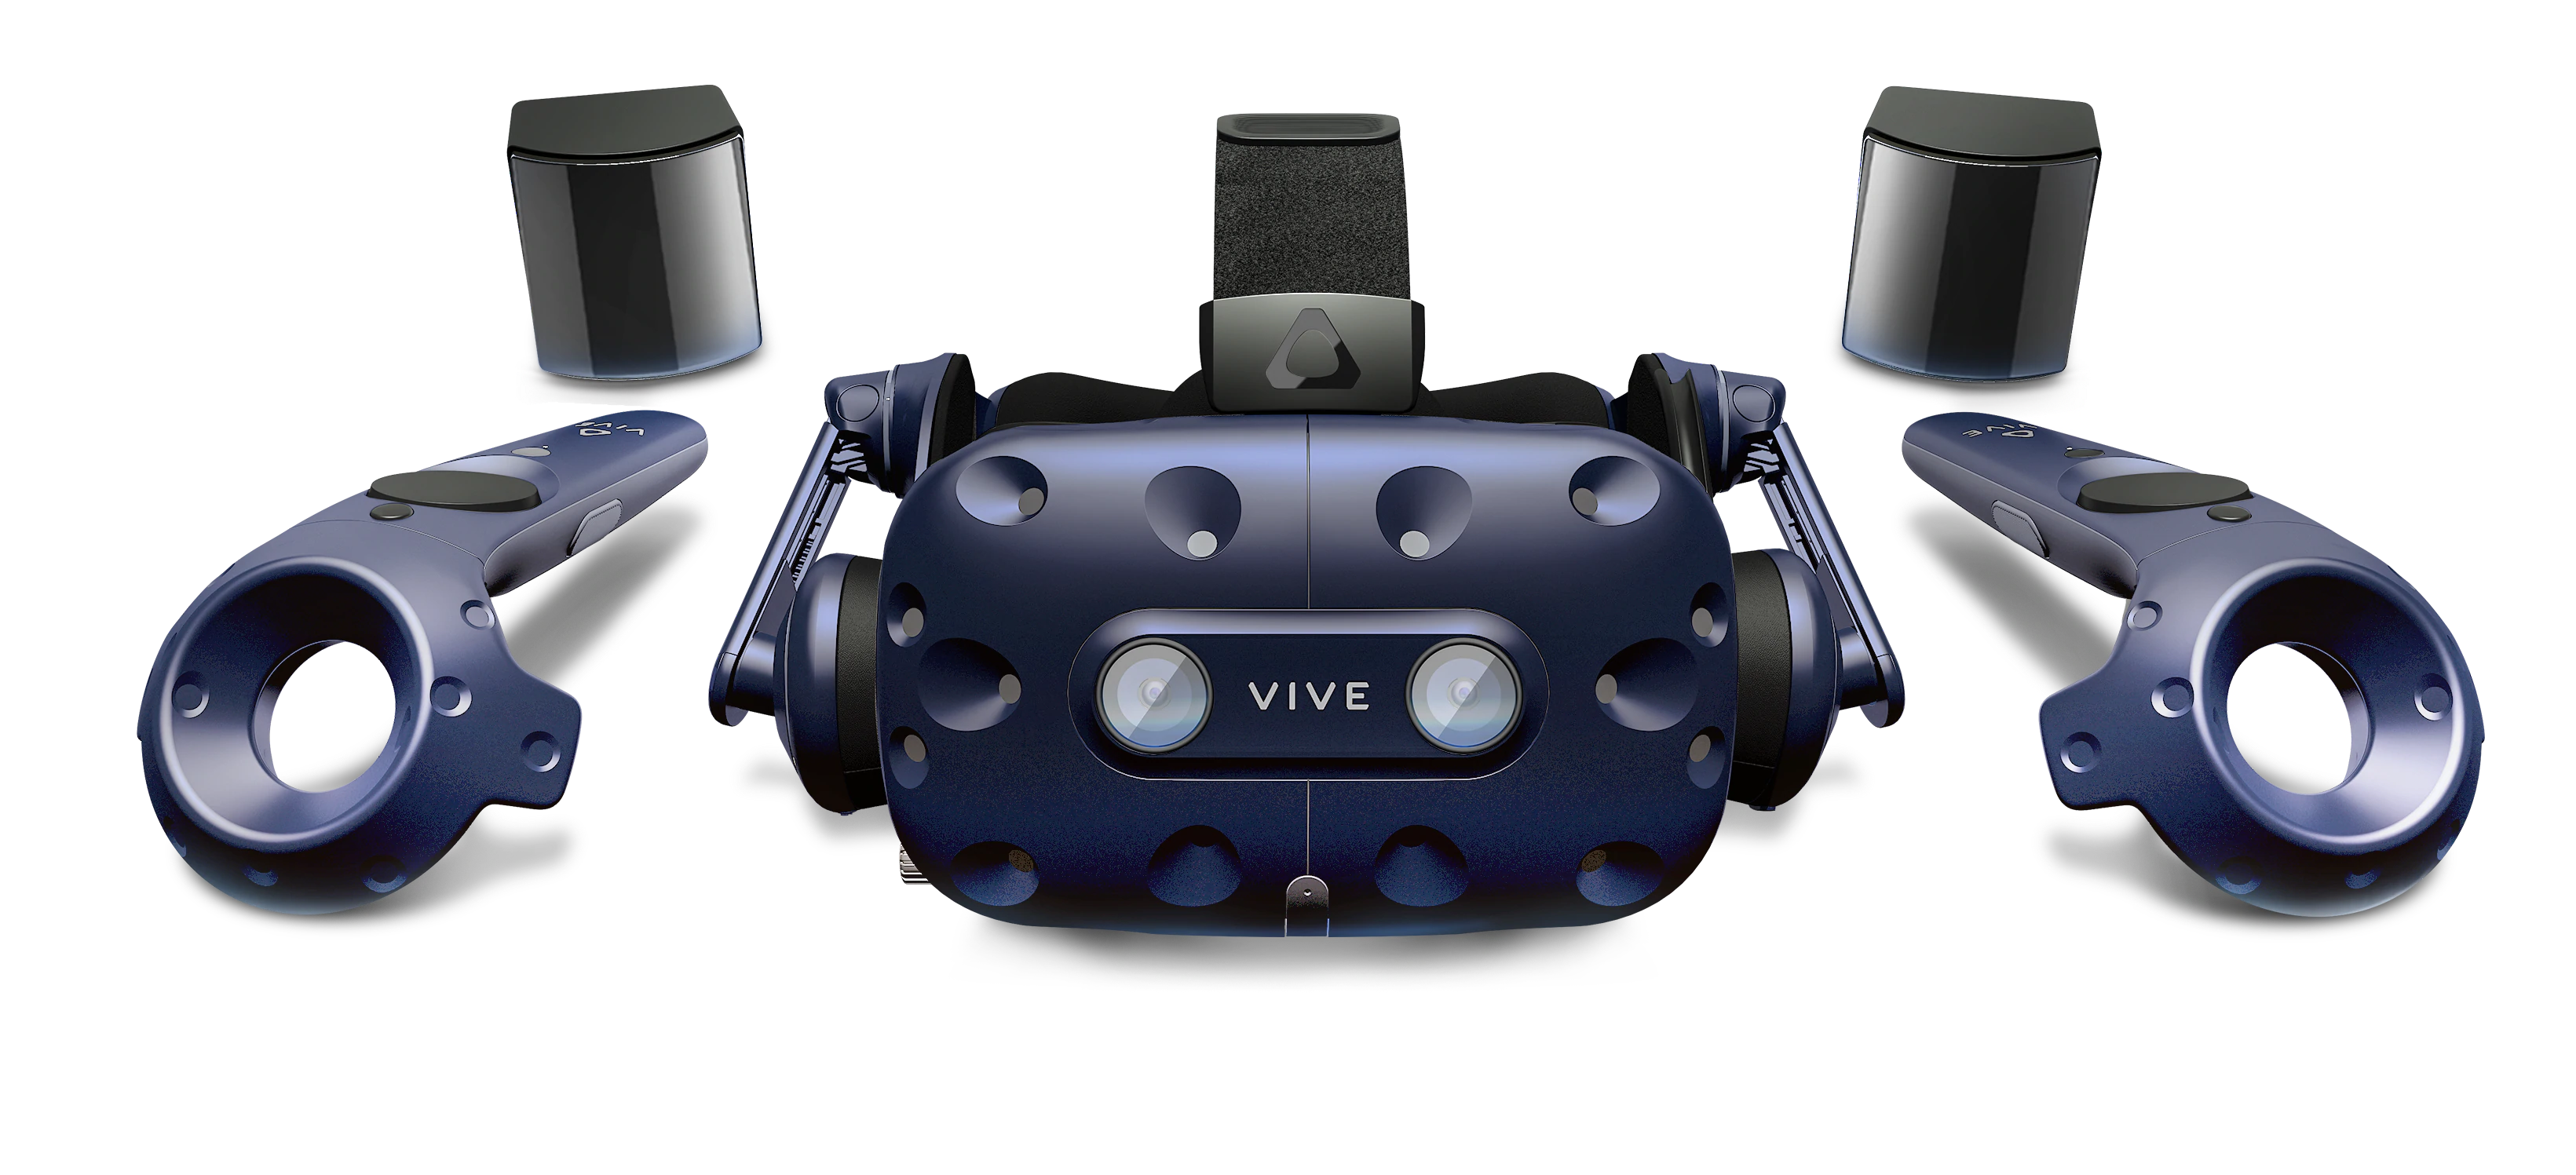
\includegraphics[width=0.7\linewidth]{Bilder/A26_Vivepro}
	\caption{VIVE Pro (mitte), Controller und Basisstationen (außen) [A26]}
	\label{fig:ViveproKit}
\end{figure}
\begin{figure}[h]
	\centering
	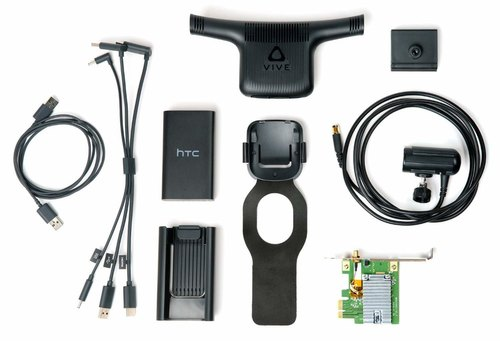
\includegraphics[width=0.5\linewidth]{Bilder/A27_WirelessKit}
	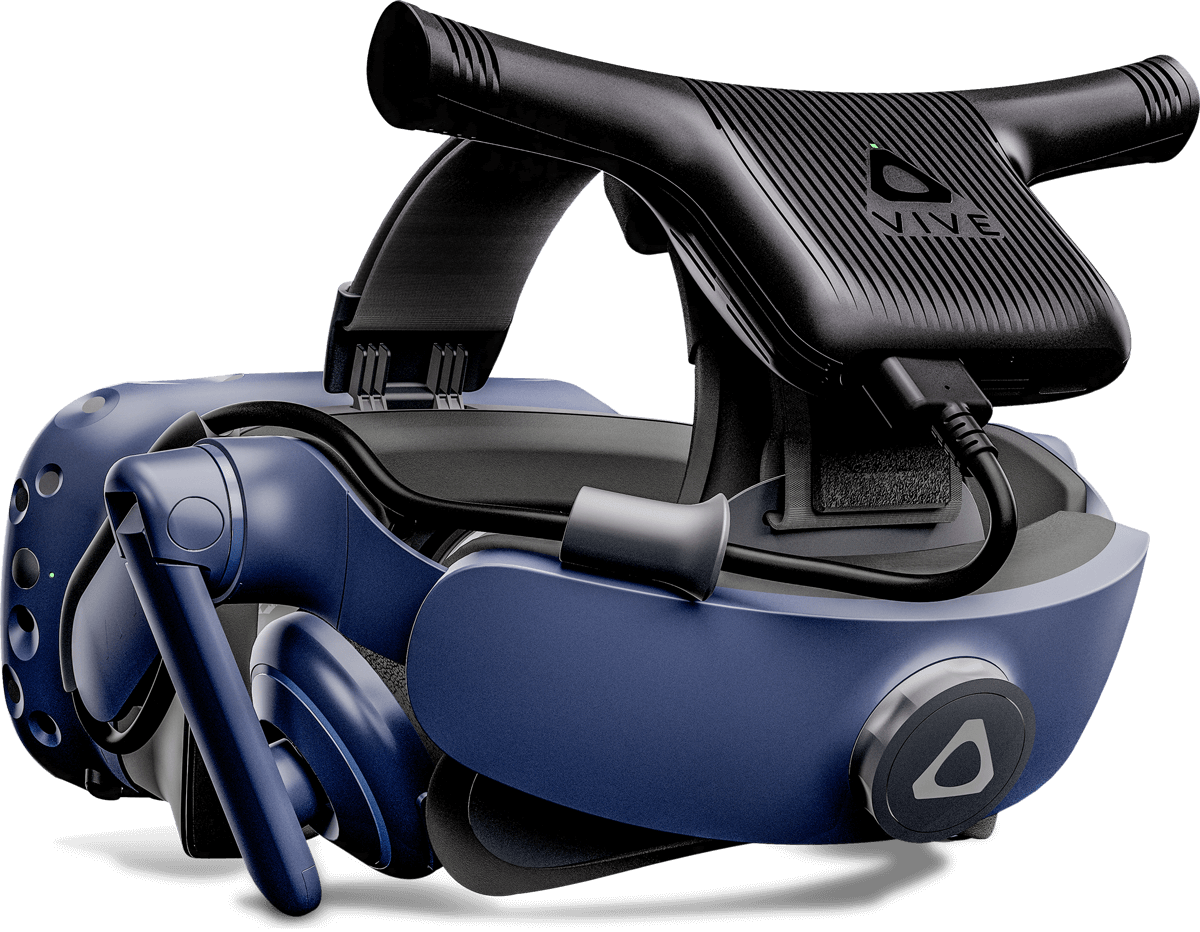
\includegraphics[width=0.4\linewidth]{Bilder/A28_Vive+Wireless}
	\caption{Links: VIVE Wireless Set, inkl. Erweiterungskarte, Sender, Empfänger, Akku, Kabeln und Befestigungen. Rechts: VR Brille mit angeschlossenem Sender. [A27+A28]}
	\label{fig:WirelessKit}
\end{figure}
Neben den außerordentlich guten technischen Spezifikationen der HTC VIVE Pro waren die \textbf{HTC VIVE Tracker} (Vgl. Abbildung \ref{fig:ViveTracker}) ein weiterer Grund warum diese VR Brille zur Umsetzung dieser Arbeit ausgewählt wurde. Die VIVE Tracker werden genauso wie die VR Brille und die dazugehörigen Controller von den Basisstationen im raum geortet und liefern ebenfalls Informationen über ihre Position und Ausrichtung im Raum. Durch den kleinen Formfaktor können die Tracker an beliebigen Objekten befestigt werden um die Bewegung dieser Objekte in der virtuellen Welt abzubilden [30, ViveTracker].
\newline
\begin{figure}[h]
	\centering
	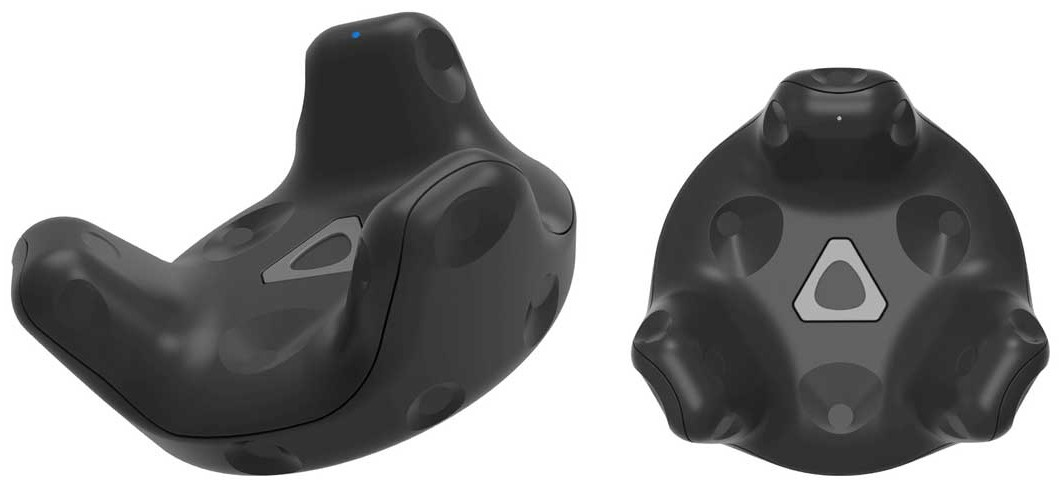
\includegraphics[width=0.5\linewidth]{Bilder/A29_ViveTracker}
	\caption{HTC VIVE Tracker [A29]}
	\label{fig:ViveTracker}
\end{figure}
\newline
Bei dieser Arbeit kamen die Tracker für die Ortung einzelner Körperteile zum Einsatz, da die Hände und der Kopf werden bereits durch die Controller und die VR Brille abgedeckt wurden. Konkret kamen die Tracker für die Ortung der Füße, der Knie, des Beckens und der Ellenbogen zum Einsatz. Durch das Schraubgewinde auf der Unterseite lassen sich die Tracker einfach befestigen. Für die Befestigungen am Becken und an den Füßen wurde auf \textbf{fertige Halterungen} zurückgegriffen (Vgl. Abbildung \ref{fig:Mounts}). Um die Tracker an den Knien und an den Ellenbogen zu befestigen habe ich mir \textbf{eigene Halterungen} gebaut (Vgl. Abbildung \ref{fig:Mounts}). Für diese Halterungen wurden handelsübliche Knie- und Ellenbogenschoner verwendet, durch die ein Loch gebohrt wurde um eine Schraube mit Hilfe einer Mutter zu fixieren. Durch das bereits erwähnte Schraubgewinde auf der Unterseite der Tracker ließen diese sich einfach an diesen Schrauben befestigen.
\begin{figure}[h]
	\centering
	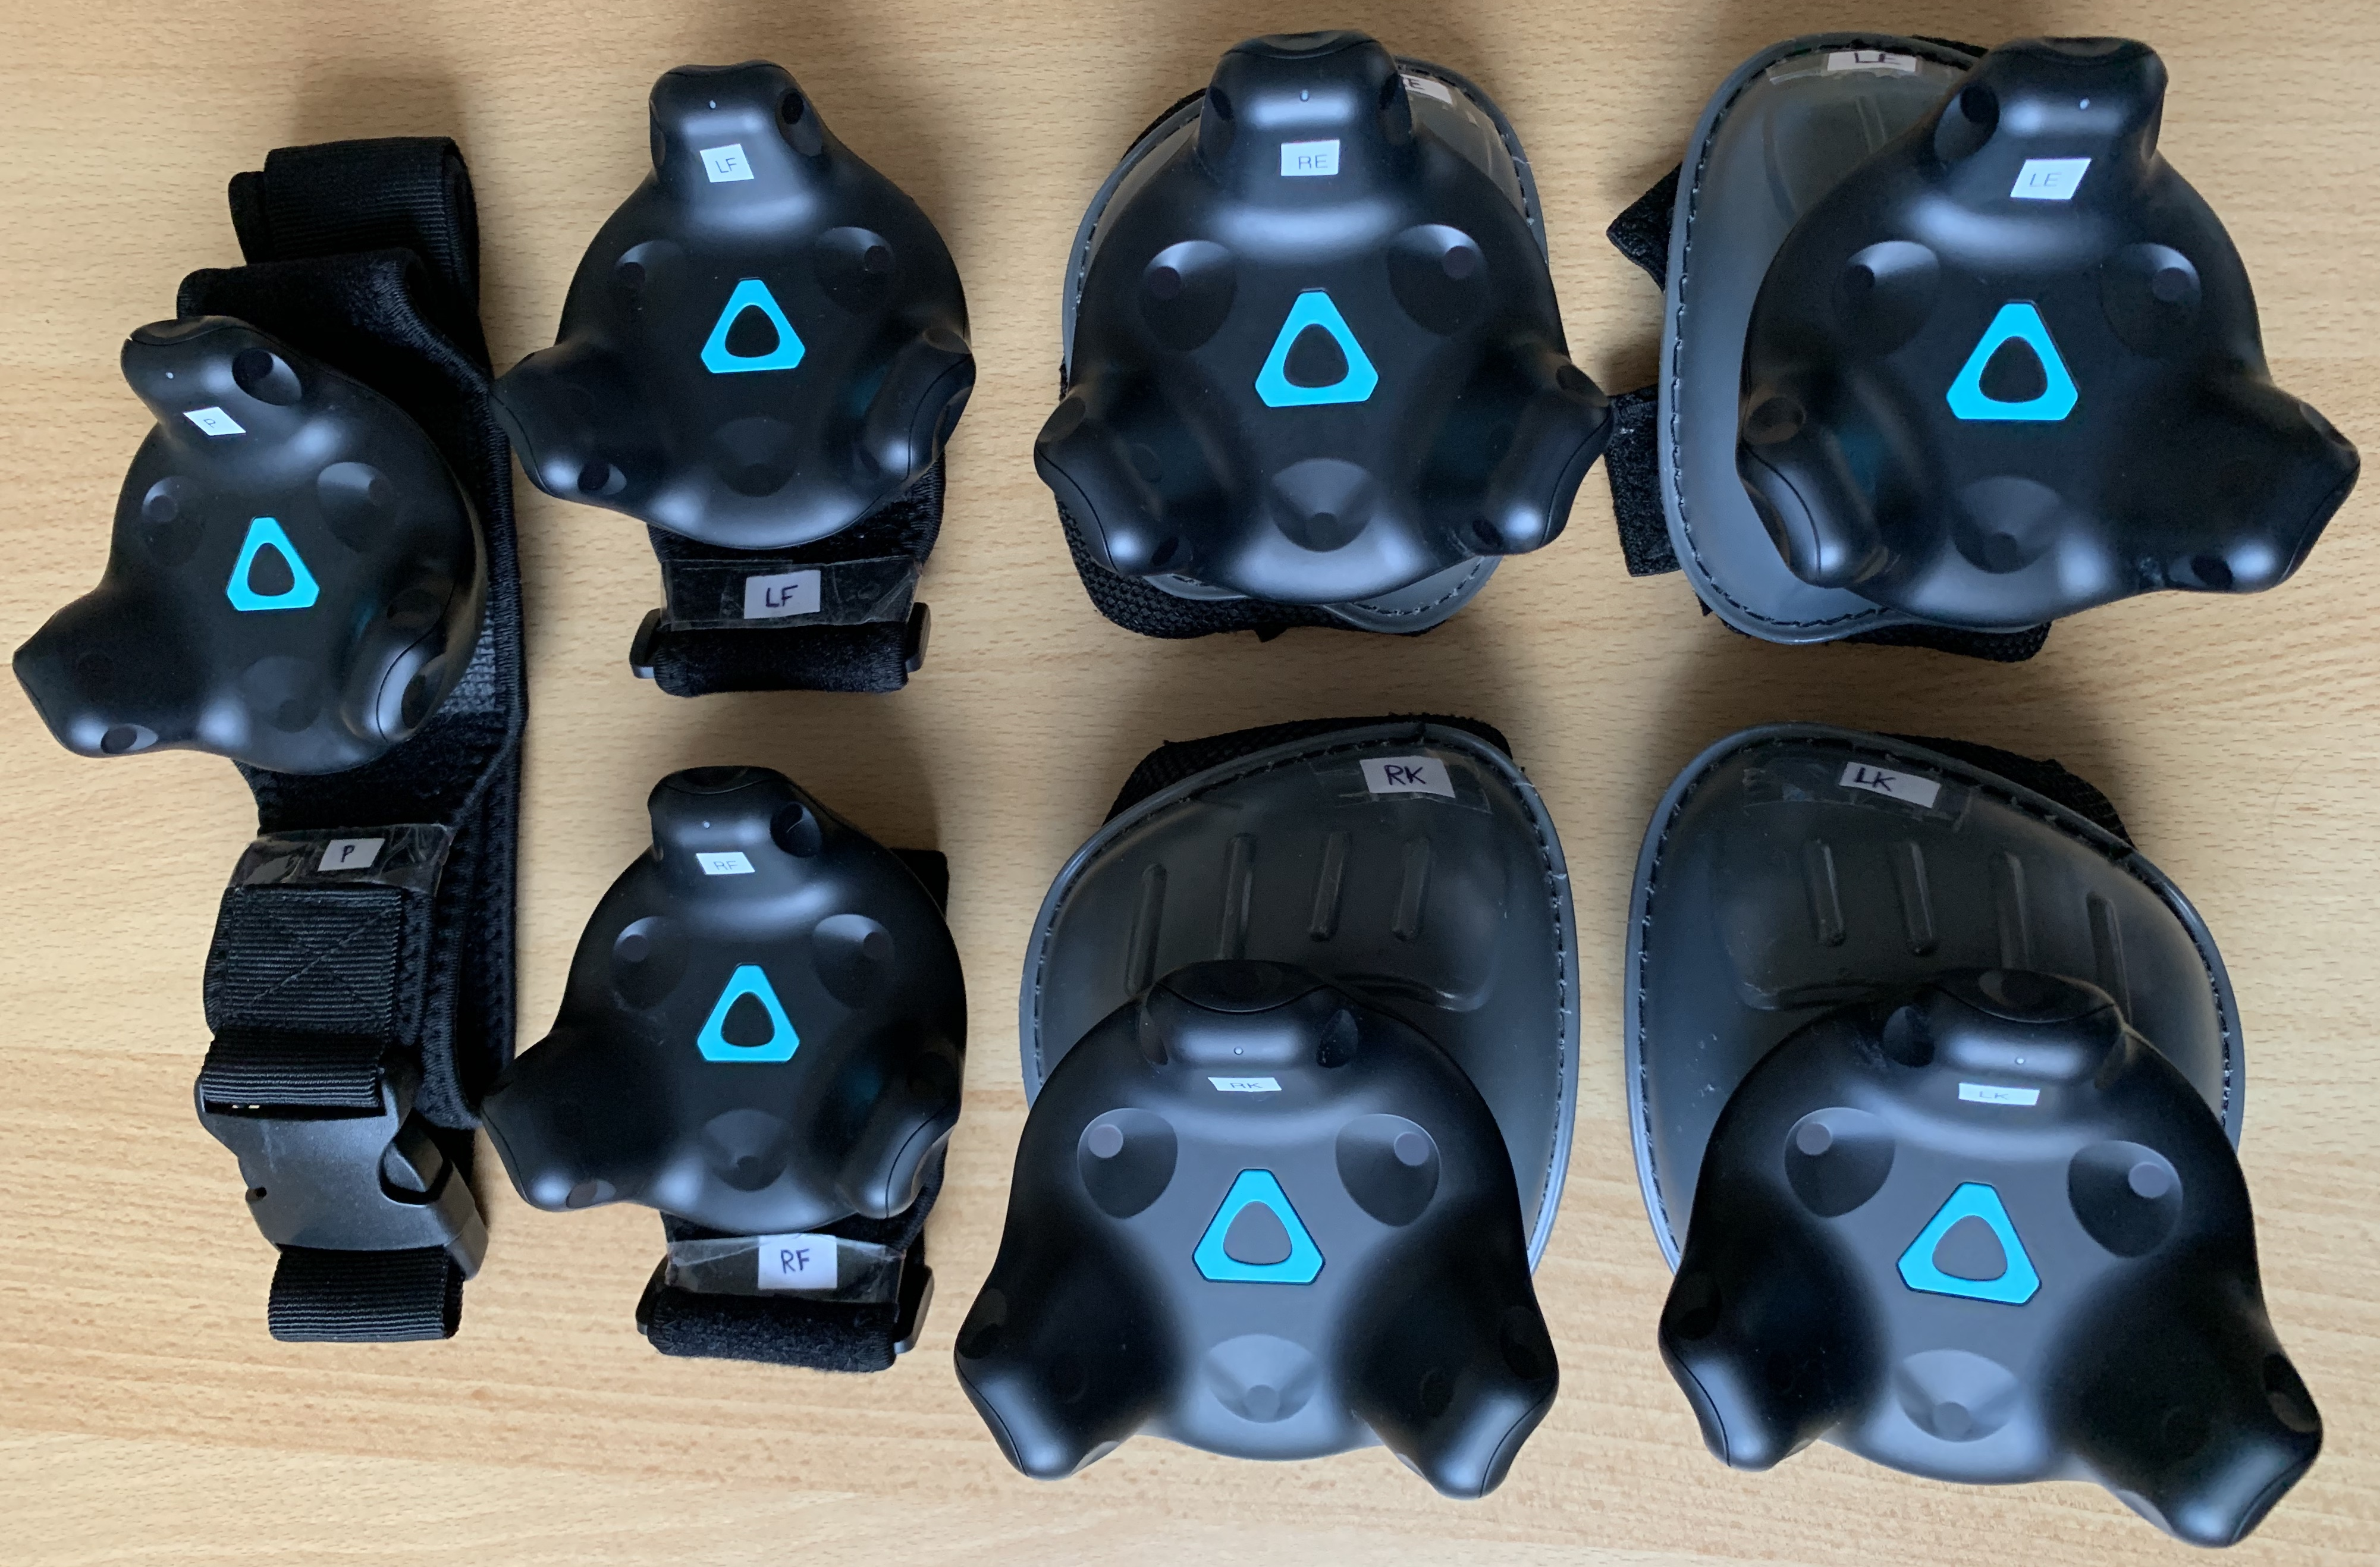
\includegraphics[width=0.7\linewidth]{Bilder/A32_Mounts}
	\caption{Gekaufte (links) und eigene (rechts) Befestigungen für die Tracker, eigene Abbildung}
	\label{fig:Mounts}
\end{figure}

%--------------------------------------------------------------------------------------------------
\section{Eingesetzte Software}\label{sec:Software}
Wie in Abbildung \ref{fig:CodeDarstellung} bereits angedeutet kamen für die Umsetzung dieses Projektes verschiedene Anwendungen und Plugins zum Einsatz. Im Folgenden werden diese genauer erläutert:

\subsection{VIVE Wireless}\label{sec:VIVEWireless}
Die VIVE Wireless Anwendung (Vgl. Abbildung \ref{fig:VIVEWirelessSteamVR}) ist für die direkte Verbindung mit der VR Hardware verantwortlich. Wie bereits in Abbildung \ref{fig:WirelessKit} dargestellt wird dafür im Computer eine Erweiterungskarte installiert, die es einem ermöglicht den entsprechenden Empfänger für die Signale am PC anzuschließen. Der in Abbildung \ref{fig:WirelessKit} dargestellte an der VR Brille montierte Sender bildet das Gegenstück zu diesem Empfänger. Diese Hardware-Erweiterung in Kombination mit der VIVE Wireless Anbindung ermöglicht die kabellose Verwendung der VR Brille.

\subsection{SteamVR}\label{sec:SteamVR}
SteamVR (Vgl. Abbildung \ref{fig:VIVEWirelessSteamVR}) stellt eine weitere wichtige Anwendung im Kontext dieser Arbeit dar. Die meisten Anwendungen für VR Brillen von unterschiedlichen Herstellern sind auf die Schnittstelle der SteamVR Software ausgelegt. Das Gegenstück zu dieser Schnittstelle bildet das SteamVR Plugin, welches im weiteren Verlauf dieses Kapitels vorgestellt wird. Falls die VR Brille ohne das VIVE Wireless Set verwendet wird, wird diese über ein Kabel direkt mit dem PC und somit direkt mit der SteamVR Anwendung verbunden. Da für diese Arbeit das VIVE Wireless Set eingesetzt wurde, wird die VR Brille indirekt über die VIVE Wireless Anwendung mit der SteamVR Anwendung verbunden. Des Weiteren bringt die SteamVR Anwendung eine große Menge an Funktionalitäten mit sich. Dazu gehören Beispielsweise die Möglichkeit den Spielraum zu vermessen oder die Tastenbelegungen der Controller zu verändern. Zusätzlich bietet SteamVR eine Art Hauptmenü an, welches über die in Kapitel \ref{sec:Hardware} angesprochene Taste aufgerufen werden kann.
\newline
Zusammenfassend lässt sich sagen, dass SteamVR eine zentrale Schnittstelle bietet mit der sich die VR Brille, die Controller, die Basisstationen und die Tracker verwalten lassen.
\begin{figure}[h]
	\centering
	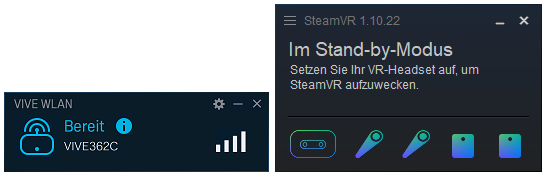
\includegraphics[width=0.8\linewidth]{Bilder/A33_VIVESteam}
	\caption{Links: VIVE Wireless, Rechts: SteamVR, eigene Abbildung}
	\label{fig:VIVEWirelessSteamVR}
\end{figure}

\subsection{Unity Engine}\label{sec:UnitEngine}
Die Unity Engine ist eine 3D-Entwicklungsumgebung und wurde für die Umsetzung dieser Arbeit verwendet. Als Programmiersprache für diese Entwicklungsumgebung kommt die Sprache C\# zum Einsatz.
\newline
Unity bietet den Vorteil in einem Projekt mehrere Szenen (Umgebungen) aufzusetzen und schnell zwischen diesen wechseln zu können. Des Weiteren können die Szenen direkt in der Anwendung bearbeitet werden wenn z.B. 3D-Modelle bearbeitet, hinzugefügt oder entfernt werden sollen. Des Weiteren bringt die Unity Engine eine Vielzahl von bereits eingebauten Funktionalitäten mit sich, die Entwicklern einiges an Arbeit ersparen können. So gibt es Beispielweise vorgefertigte Elemente für grafische Benutzeroberflächen oder sogar ein eingebautes Physiksystem mit dem sich z.B. Kollisionen von Objekten leicht abfragen können. Dank des eingebauten Asset Stores („Marktplatz“) lassen sich in einem internen Marktplatz dank der großen Entwickler-Community aus einer großen Auswahl an Erweiterungen, Texturen, Modelle, etc. beliebig viele Komponenten herunterladen und im eigenen Projekt einfügen. Aufgrund dessen kann man sagen, dass Unity als Entwicklungsumgebung den Entwicklern ermöglicht Modularität in Ihren Projekten umzusetzen.
\newline
Auch bei dieser Arbeit kamen Erweiterungen aus dem Asset Store zum Einsatz. Neben vereinzelten Texturen aus dem Asset Store sind die wichtigsten Erweiterungen das SteamVR und das Final IK Plugin, welche im Folgenden genauer erläutert werden.

\subsubsection{SteamVR Plugin für die Unity Engine}\label{sec:SteamVRPlugin}
Das SteamVR Plugin bildet wie bereits erwähnt und in Abbildung XX illustriert das Gegenstück zur SteamVR Anwendung und vollendet die Schnittstelle zwischen Unity und der VR Hardware. Des Weiteren bietet das Plugin eine große Menge an vorgefertigten Funktionalitäten, wie z.B. das in Abbildung \ref{fig:CodeDarstellung} angedeutete SteamVRTrackedObject Skript.

\subsubsection{Final IK Plugin für die Unity Engine}\label{sec:FinalIKPlugin}
Ein weiteres wichtiges Plugin ist das Final IK Plugin von dem Entwickler RootMotion. Das IK im Namen des Plugins steht für Inverse Kinematics (deutsch: Inverse Kinematik), also „aus vorhandenen Koordinaten Gelenkwinkel berechnen“ [31, Ham., S.20]. Im Kontext dieser Arbeit bedeutet dies, dass mit Hilfe der gelieferten Koordinaten der Tracker die entsprechenden Gelenkwinkel für die Körperteile berechnet werden. Neben diesen Berechnungen liefert das Final IK Plugin noch das eigentliche Modell des Menschen und einige weitere Funktionalitäten, wie z.B. die Kalibrierung des Modells.

%--------------------------------------------------------------------------------------------------
\section{Das Menschmodell}\label{sec:DasMenschmodell}
In diesem Abschnitt zunächst wird der Aufbau und der Nutzen des Menschmodells ohne die Interaktionsschnittstelle erläutert, da diese beiden Komponenten aufgrund der Anforderungen an die Modularität unabhängig voneinander implementiert wurden.

\subsection{Der Aufbau des Menschmodells}\label{sec:MMAufbau}
Das entstandene Menschmodell basiert auf dem durch das Final IK Plugin gelieferten Modells. Im Folgenden werden die einzelnen Komponenten erläutert. Zu den Komponenten gehören das eigentliche Modell, die Skripte und die ergänzenden Komponenten die durch dieser Arbeit dazugekommen sind.

\subsubsection{Das eigentliche Modell}\label{sec:MMModell}
Das Final IK Plugin liefert mehrere Modelle. Für diese Arbeit wurde das Modell mit dem Namen Dummy ausgewählt, welches wie der Name bereits vermuten lässt wie ein Crashtest-Dummy aussieht (Vgl. Abbildung \ref{fig:Dummy}).
\newline\newline
Das Modell in der Szene trägt den Namen \textbf{Dummy} und enthält das sogenannte \textbf{VR IK Skript} des Final IK Plugins. Dieses Skript kümmert sich um die Animation des Modells, daher sind Referenzen zu allen Körperteilen gesetzt. Zu den Körperteilen Kopf, Hände und Füße gibt es zusätzliche Einstellungsmöglichkeiten. Um den Dummy zu verwenden müssen mindestens der Kopf und die beiden Hände als \textbf{Targets} (Ziele für das Tracking) gesetzt werden. Optional können auch die Füße als Targets gesetzt werden. Falls man die Genauigkeit des Trackings um noch eine Stufe verbessern möchte, kann man sogenannte \textbf{Bend Goals} („Beug-Ziele“) setzen (Vgl. Abbildung \ref{fig:TargetBendGoal}). Es gibt insgesamt fünf solcher Bend Goals. Bei dem Kopf ist das zugehörige Bend Goal der Steißbein-Tracker, bei den Händen die Ellenbogen-Tracker und bei den Füßen die Knie-Tracker. Die Targets und Bend Goals werden von dem Skript TrackerAssignment verwaltet, welches im weiteren Verlauf dieses Kapitels erläutert wird.
\begin{figure}[h]
	\centering
	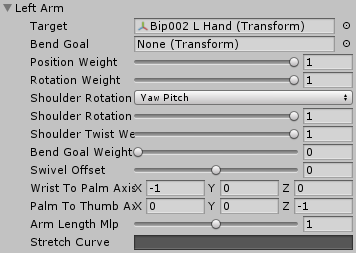
\includegraphics[width=0.4\linewidth]{Bilder/A36_TargetsBendGoals}
	\caption{Targets und Bend Goal am Beispiel des linken Arms, eigene Abbildung}
	\label{fig:TargetBendGoal}
\end{figure}
\newline
Des Weiteren enthält das Objekt Dummy mit dem VR IK Skript zwei weitere Kind-Objekte (Vgl. Abbildung \ref{fig:Dummy}), den \textbf{BipDummy} und den gleichnamigen \textbf{Dummy}. Letzterer ist nur der Skinned-Mesh-Renderer und kümmert sich darum, dass die Texturen der Körperteile gerendert werden. Dies bietet den Vorteil, dass man leicht durch neue Texturen das aussehen des Dummy verändern kann. Das Objekt BipDummy enthält die Transformationen, also Position, Rotation und Skalierung aller Körperteile. Dieser Modulare Aufbau ermöglicht es einem das Menschmodell in Zukunft durch beliebige neue Modelle auszutauschen, solange die Transformationen für die Körperteile Füße, Knie, Steißbein, Hände, Ellenbogen und Kopf vorhanden sind.
\begin{figure}[h]
	\centering
	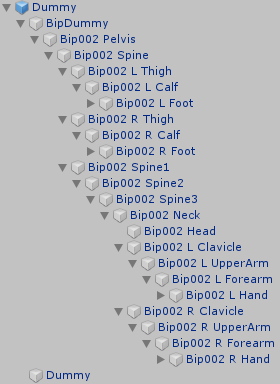
\includegraphics[width=0.4\linewidth]{Bilder/A34_DummyAufbau}
	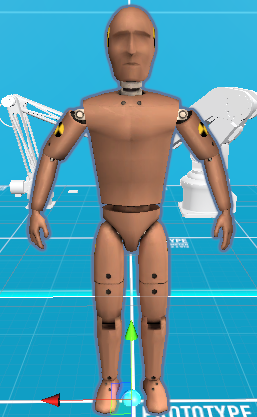
\includegraphics[width=0.338\linewidth]{Bilder/A35_Dummy}
	\caption{Final IK Dummy Modell, eigene Abbildung}
	\label{fig:Dummy}
\end{figure}

\subsubsection{Ergänzende Komponenten}\label{sec:MMKomponenten}
Um das Menschmodell einsatzfähig für die VR Hardware zu machen mussten noch zwei weitere Komponenten zu dem eigentlichen Modell hinzugefügt werden. Diese Komponenten sind das SteamVR CameraRig und die Targets (Ziele) für die optionalen Tracker.
\newline\newline
Das \textbf{SteamVR CameraRig} (Vgl. Abbildung \ref{fig:CameraRig}) ist eine von SteamVR zur Verfügung gestellte Komponente zur Eingrenzung des Spielbereichs und Tracking der Controller (Hier: Hände) und der VR-Brille (Hier: Kopf). Die Komponente besteht aus den drei Kind-Objekten Controller (left), Controler (right) und Camera. Controller (left) und Controller (right) enthalten zusätzlich das 3D-Modell des Controllers als Kind-Objekt, um diesen in der virtuellen Welt anzeigen zu können. 
\newline
Durch diese drei Objekte werden die Bewegungen der beiden Controller und des Kopfes in der virtuellen Welt wiedergespiegelt. Des Weiteren ist es wichtig zu erwähnen, dass das CameraRig für diese Arbeit modifiziert wurde. Den beiden Controllern und der Kamera wurden Kopien der Transformationen der beiden Hände und des Kopfes als Kind-Objekte hinzugefügt. Diese Kopien kamen beim VR IK Skript zum Einsatz um Informationen über die Positionen der Hände und des Kopfes zu erhalten (Vgl. Abbildung \ref{fig:TargetBendGoal}), da diese sich als Kind-Objekte der Controller (Hier: Hände) und der Kamera (Hier: Kopf) entsprechend mitbewegen.
\newline
Abschließend sei noch zu erwähnen, dass die Transformation vom Kopf (Bip002 Head) um ca. -0,113 Einheiten entlang der Y- und Z-Achse gegenüber dem Parent-Objekt Camera verschoben wurde, damit die Kamera sich nicht innerhalb des Kopfes des Modells befindet. Die Transformationen von der linken (Bip002 L Hand) und der rechten (Bip002 R Hand) Hand wurden nicht verschoben.
\begin{figure}[h]
	\centering
	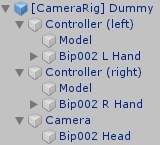
\includegraphics[width=0.25\linewidth]{Bilder/A37_CameraRig}
	\caption{Modifiziertes CameraRig, eigene Abbildung}
	\label{fig:CameraRig}
\end{figure}
\newline
Die zweite wichtige ergänzte Komponente sind die sogenannten \textbf{Targets} (Ziele) (Vgl. Abbildung \ref{fig:Targets}). Da nur sichergestellt ist, dass der Kopf und die Hände durch die VR-Brille und die Controller mit Hilfe des SteamVR CameraRigs verfolgt werden bedarf es zusätzliche Verfolgungsziele für die optionalen Tracker an den Füßen, Knien, Ellenbogen und dem Steißbein.
\newline
Die Targets enthalten momentan noch jeweils ein Kind-Objekt (Vgl. Abbildung \ref{fig:Targets}). Diese Objekte sind lediglich für den Entwicklungsprozess gedacht und können auf Wunsch einfach gelöscht werden, da es sich nur um einfache gefärbte Kugeln handelt, die dem Entwickler anzeigen wo die Tracker sich momentan im Raum befinden. 
\newline
Des Weiteren kommen die Targets genauso wie die Transformationen der Hände und des Kopfes im CameraRig beim VR IK Skript zum Einsatz, um dem Skript Informationen über die Positionen der entsprechenden Körperteile zu liefern. Dabei ist anzumerken, dass die Füße und das Steißbein als eigentliche Targets (Ziele) zum Einsatz kommen, während die Knie und die Ellenbogen als Bend Goals („Beug-Ziele“) verwendet werden (Vgl. Abbildung \ref{fig:TargetBendGoal}).
\begin{figure}[h]
	\centering
	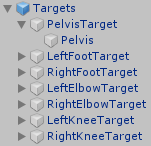
\includegraphics[width=0.25\linewidth]{Bilder/A38_Targets}
	\caption{Targets, eigene Abbildung}
	\label{fig:Targets}
\end{figure}
\newline
Jedes dieser Targets enthält wie bereits in Abbildung \ref{fig:CodeDarstellung} illustriert das Skript \textbf{SteamVR Tracked Object} (Vgl. Abbildung \ref{fig:TrackedObject}). Durch das bereits erwähnte Skript TrackerAssignment wird jedem der Targets der Index des zugehörigen Trackers zugewiesen. Die Standardeinstellung ist „none“, da das Menschmodell auch ohne jegliche dieser optionalen Tracker und sogar nur mit einer beliebigen Teilmenge von ihnen funktioniert.
\begin{figure}[h]
	\centering
	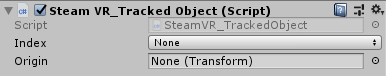
\includegraphics[width=0.45\linewidth]{Bilder/A39_SteamVRTrackedObject}
	\caption{SteamVR Tracked Object Komponente, eigene Abbildung}
	\label{fig:TrackedObject}
\end{figure}

\subsubsection{Ergänzender Code}\label{sec:MMCode}
Für das eigentliche Menschmodell ohne die Interaktionsschnittstelle kommen wie bereits in Abbildung \ref{fig:CodeDarstellung} dargestellt zwei weitere Klassen zum Einsatz. Diese beiden Klassen tragen die Namen CalibrationController und TrackerAssignment.
\newline\newline
Die Klasse \textbf{TrackerAssignment} (Vgl. Abbildung \ref{fig:MenschUML}) kümmert sich wie bereits erwähnt um die Zuweisung der Tracker zu den entsprechenden Körperteilen. Aufgrund dessen enthält diese Klasse in öffentlichen Variablen Verweise auf alle SteamVR Tracked Object Skripte der optionalen Tracker sowie die Transformationen der zugehörigen Körperteile. Des Weiteren enthält diese Klasse in öffentlichen Variablen Verweise auf den Calibration Controller und das VR IK Skript vom Dummy. Außerdem enthält diese Klasse noch einige private Variablen, insbesondere die bereits in Kapitel \ref{sec:Variablendefinition} erwähnten IDs der verschiedenen Tracker.
\newline
Insgesamt enthält diese Klasse zwei Methoden. Die erste Methode trägt den Namen Start und wird wie der Name bereits vermuten lässt einmal bei der Initialisierung ausgeführt und danach nie wieder. In dieser Methode werden lediglich ein paar Variablen die im späteren Verlauf verwendet werden deklariert. Die zweite Methode trägt den Namen AssignTrackers und beinhaltet die gesamte Funktionalität dieser Klasse.
\newline
Zunächst werden mittels einer Schleife alle angeschlossenen Geräte durchlaufen und mit den hinterlegten IDs der Tracker verglichen. Sobald die ID von einem der angeschlossenen Geräte mit einer der hinterlegten IDs übereinstimmt, wird dem SteamVR Tracked Object Skripts des Targets des entsprechenden Körperteils der Index dieses Trackers zugewiesen (Vgl. Abbildung \ref{fig:TrackedObject}).
\newline
Daraufhin werden dem Calibration Controller die Referenzen zu den Transformationen der Füße und des Steißbeins übergeben (Vgl. Abbildung \ref{fig:CodeDarstellung}), falls die entsprechenden Tracker aktiv sind. Es ist anzumerken, dass jede beliebige Teilmenge dieser drei Tracker aktiv sein kann, ohne das Ergebnis der Kalibrierung zu verschlechtern.
\newline
Anschließend werden durch den Verweis auf das VR IK Skript die Bend Goals zugewiesen, falls die Tracker für die Knie und Ellenbogen angeschlossen sind. Dafür muss zusätzlich das Bend Goal Weight (die Gewichtung des Bend Goals) auf den Wert 1 gesetzt werden (Vgl. Abbildung \ref{fig:TargetBendGoal}). Hier ist ebenfalls anzumerken, dass jede beliebige Teilmenge der Tracker aktiv sein kann, ohne das Ergebnis der Darstellung des Menschmodells wesentlich zu verschlechtern. Falls Beispielsweise der Tracker am linken Ellenbogen aktiv ist aber der Tracker am rechten Ellenbogen nicht, wird die Position des rechten Ellenbogens einfach durch das VR IK Skript anhand der Ausrichtung der Hand und des gesamten Körpers automatisch approximiert.
\newline\newline
Die Klasse \textbf{CalibrationController} (Vgl. Abbildung \ref{fig:MenschUML}) arbeitet mit dem bereits vorhandenen VR IK Calibrator des Final IK Plugins. Aufgrund dessen enthält die Klasse in öffentlichen Variablen die Verweise auf das VR IK Skript vom Dummy, auf die Transformationen vom Kopf und den beiden Händen und auf die Klasse TrackerAssignment. Des Weiteren enthält die Klasse die öffentlichen Variablen Settings (Einstellungen) und Data (Daten der Kalibrierung). Schließlich enthält die Klasse noch öffentliche aber noch nicht initialisierte Variablen für die Verweise auf die Transformationen des Steißbeins und der beiden Füße.
\newline
Insgesamt enthält die Klasse drei Methoden, wobei die letzte den Namen LateUpdate trägt und in der Regel nicht verwendet wird. Diese Klasse ist nur für Entwicklungszwecke da und war in einer Demo-Klasse des Final IK Plugins vorhanden. Sie ermöglicht es einem die Kalibrierung des Dummys durch das drücken einer bestimmten Taste auf der Tastatur zu starten. Die erste Methode dieser Klasse trägt den Namen Update und wird einmal pro Frame ausgeführt. Aufgabe dieser Methode ist es, sobald vom Bediener die entsprechende Taste am linken Controller gedrückt wird den Kalibrierungsprozess durch die zweite Methode der Klasse mit dem Namen Calibrate zu starten. Es ist anzumerken, dass der Kalibrierungsprozess beliebig oft ausgeführt und somit nach Bedarf erneuert werden kann.
\newline
In der Methode Calibrate wird zunächst durch den Verweis auf die Klasse TrackerAssignment die Zuweisung der einzelnen Tracker gestartet. Hierbei ist anzumerken, dass wie bereits vorher erwähnt und in Abbildung \ref{fig:CodeDarstellung} dargestellt die noch nicht initialisierten Variablen für die Verweise auf die Transformationen des Steißbeins und der beiden Füße initialisiert werden, falls die entsprechenden Tracker angeschlossen sind. Ansonsten werden für die Kalibrierung lediglich die Positionen der Hände und des Kopfes berücksichtigt. In jedem Fall werden für die Kalibrierung die Positionen der Knie und der Ellenbogen nicht berücksichtigt.
\newline
Schließlich wird der eigentliche Kalibrierungsprozess durch die gleichnamige Methode Calibrate der Klasse VR IK Calibrator gestartet, indem die entsprechenden Variablen an diese Methode übergeben werden. Die vorher angesprochenen Variablen Settings und Data sind dafür da, falls man mit Hilfe der Klasse VR IK Calibrator und deren Methoden Kalibrierungen abspeichern und wieder laden möchte. Diese Funktionalität wurde für diese Arbeit nicht berücksichtigt.
\begin{figure}[h]
	\centering
	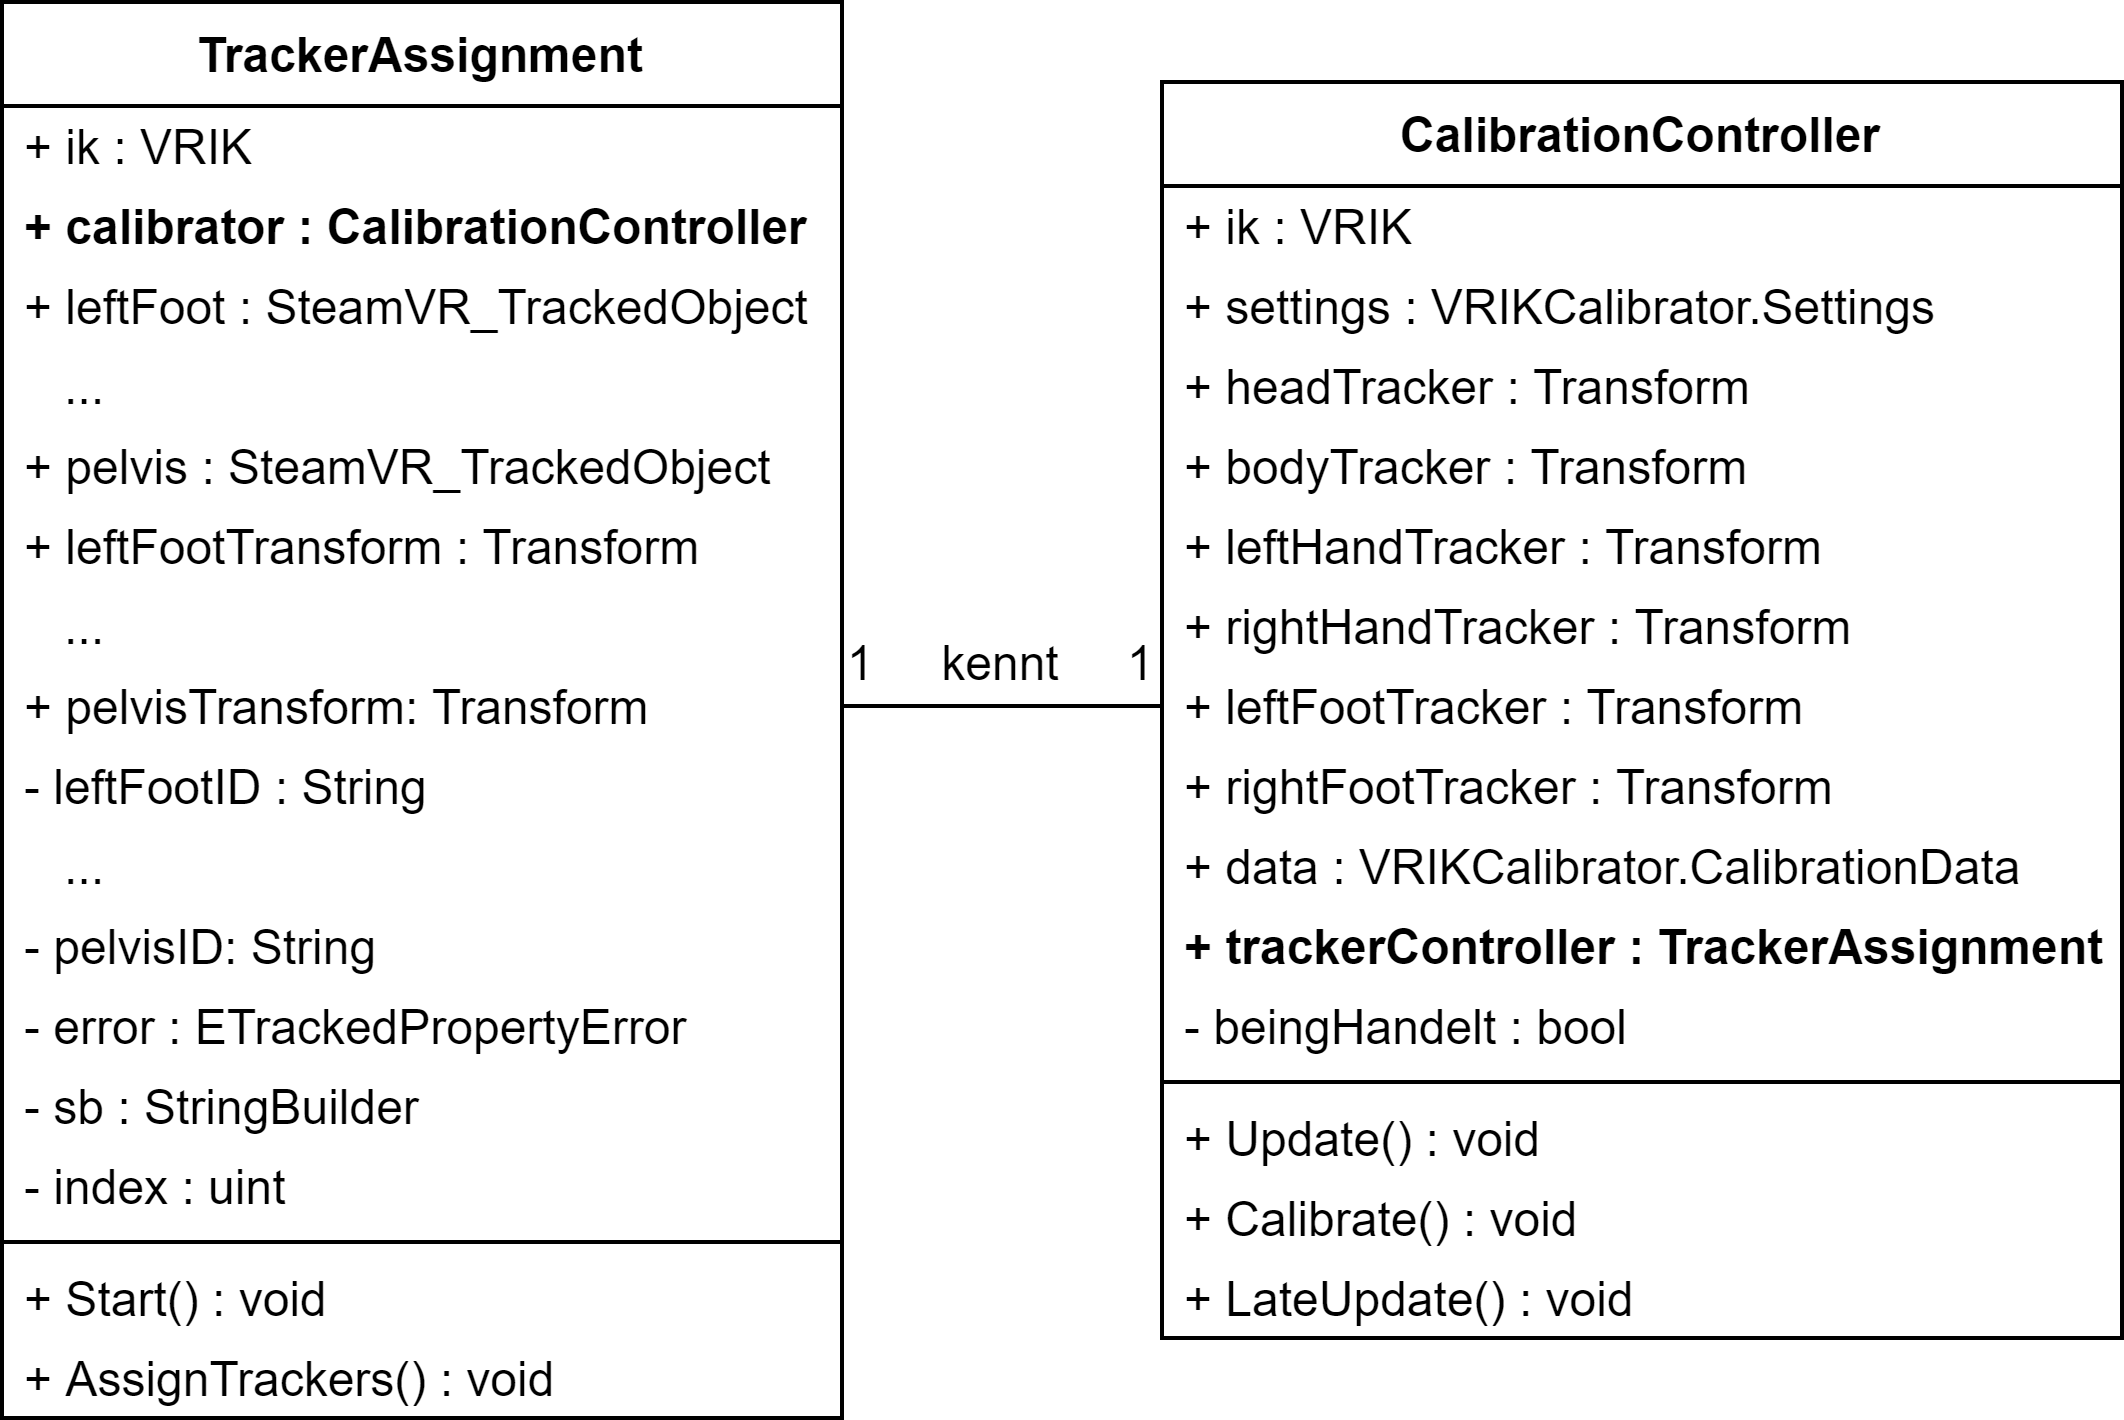
\includegraphics[width=0.65\linewidth]{Bilder/A40_MenschUML}
	\caption{UML Diagramm der Klassen TrackerAssignment und CalibrationController, eigene Abbildung}
	\label{fig:MenschUML}
\end{figure}

\subsection{Zusammenfassung des Menschmodells}\label{sec:MMFunktionen}
Das Menschmodell ermöglicht eine Abbildung der Bewegungen des Bedieners auf einen virtuellen Klon. Dabei müssen mindestens die VR Brille und die Controller verwendet werden, um die Positionen der Hände und des Kopfes abbilden zu können. Die Bewegungen der restlichen Körperteile werden in diesem Fall durch das VR IK Skript approximiert. Des Weiteren ermöglicht dieses Menschmodell mit Hilfe der in Abbildung XX dargestellten Befestigungen den Einsatz der HTC VIVE Tracker, um die Bewegungen der Füße, der Knie, der Ellenbogen und des Steißbeins zu berücksichtigen und somit ein genaueres virtuelles Abbild der Bewegungen zu erhalten. Es ist anzumerken, dass nicht jeder dieser Tracker aktiv sein muss und sogar jede beliebige Teilmenge dieser optionalen Tracker aktiv sein kann. Damit wird die in Kapitel XX gestellte Anforderung an die Genauigkeit erfüllt. Dadurch, dass die Abbildung der Bewegungen auf den virtuellen Klon in nahe zu Echtzeit stattfindet, wird die in Kapitel XX gestellte Anforderungen Echtzeit ebenfalls erfüllt. Außerdem ist noch anzumerken, dass durch den Kalibrierungsprozess das Menschmodell durch einen einfachen Knopfdruck an die Körpergröße von dem Bediener angepasst werden kann. Schließlich ist anzumerken, dass aufgrund des Modularen Aufbaus des Menschmodells zukünftige Erweiterungen ermöglicht werden und somit die in Kapitel XX geforderte Modularität erfüllt wird. Da das Modell zusätzlich nicht von seiner virtuellen Umgebung abhängig ist und somit in jeder beliebigen Umgebung eingesetzt werden kann wird auch die Anforderung an die Interoperabilität aus Kapitel XX erfüllt.
%--------------------------------------------------------------------------------------------------
\section{Die Interaktionsschnittstelle}\label{sec:DieInteraktionsschnittstelle}
Da das Menschmodell ohne die Möglichkeit mit der Umgebung zu interagieren nur bedingt nützlich ist, wird in diesem Abschnitt der Aufbau und der Nutzen der Interaktionsschnittstelle erläutert. Die Grundidee der Interaktionsschnittstelle ist es das Menschmodell durch einen Pointer (Zeiger) zu erweitern und somit eine intuitive Interaktion mit der Umgebung zu ermöglichen (Vgl. Abbildung XX).
\begin{figure}[h]
	\centering
	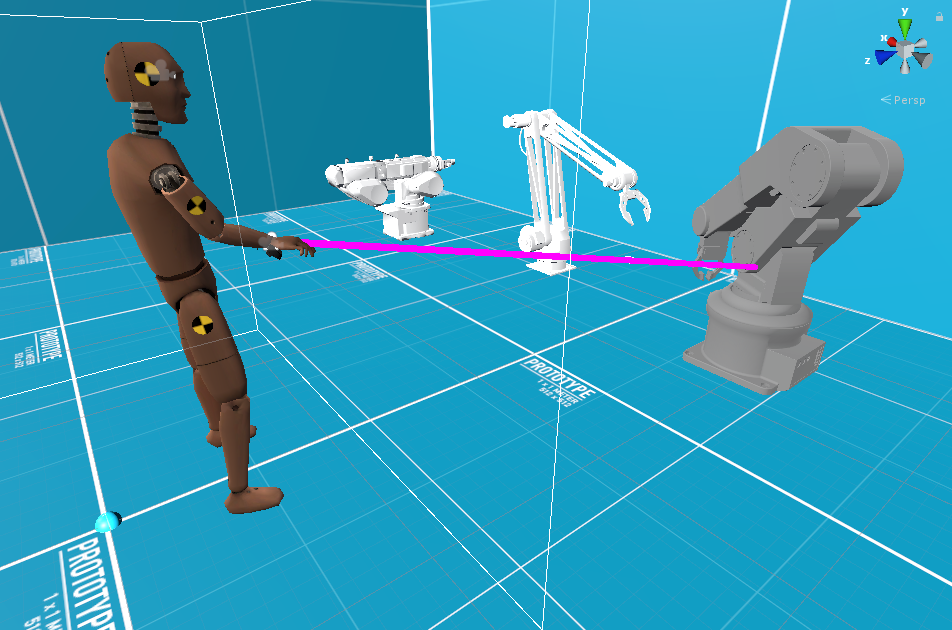
\includegraphics[width=0.65\linewidth]{Bilder/A44_InteraktionsBeispiel}
	\caption{Grundidee der Interaktion, eigene Abbildung}
	\label{fig:InteraktionBeispiel}
\end{figure}

\subsection{Der Aufbau der Interaktionsschnittstelle}\label{sec:AufbauInteraktion}
Im Folgenden zunächst das Grundgerüst der Interaktionsschnittstelle erklärt, bevor die zusätzlichen Funktionalitäten erläutert werden.

\subsubsection{Das Grundgerüst der Interaktionsschnittstelle}\label{sec:GrundgerüstInteraktion}
Das Grundgerüst der Interaktionsschnittstelle besteht lediglich aus dem Interaktionssystem, den Pointern, der Klasse die den Wechsel zwischen den beiden Pointern durchführt und der Klasse die das Menü des angeklickten Objektes aufruft. Es wurden zwei Pointer verwendet, da der eine Pointer genutzt wird um mit Objekten wie z.B. Robotern in der Umgebung zu interagieren, während der andere Pointer dafür da ist um mit Menüs zu interagieren. Es ist anzumerken, dass die Klassen VR Input für das Interaktionssystem und VR Canvas Pointer und VR Physics Pointer für die beiden Pointer auf Anleitungen des Youtube Kanals VR with Andres basieren [32, VRWithAndrew].
\newline\newline
Das \textbf{Interaktionssystem} (Vgl. Abbildung XX) basiert auf dem sogenannten Event System von Unity, welches standardmäßig in jeder Szene vorhanden ist. Mit Hilfe des Event Systems werden in der Regel der Input der Tastatur und der Maus gehandhabt. Das Event System wird für diese Arbeit durch die Klasse \textbf{VR Input} erweitert. Die Klasse enthält die drei öffentlichen Variablen eventCamera, clickButton und clickAction. Die Variable eventCamera erhält einen Verweis auf die Kamera des aktuell genutzten Pointers, während die Variablen clickButton und clickAction lediglich genutzt werden um Input-Taste zu deklarieren.
\newline
Insgesamt enthält die Klasse fünf Methoden. Die erste Methode trägt den Namen Awake, dient lediglich zur Initialisierung und wird automatisch ausgeführt sobald eine der Methoden in der Klasse ausgeführt wird. Die nächsten vier Methoden sind dafür da um den Input der Maus zu überschreiben. Die erste dieser vier Methoden trägt den Namen GetMouseButton und liefert Informationen darüber ob Taste gedrückt und wieder losgelassen wurde. Die Methoden GetMouseButtonDown und GetMouseButtonUp ermöglichen es dem Entwickler separat abzufragen, ob die Taste runtergerückt oder losgelassen wurde. Somit wird durch das Klicken der entsprechenden Taste am rechten Controller das Klicken mit der Maus simuliert. Die letzte Methode trägt den Namen mousePosition und überschreibt die Position der Maus durch den exakten Mittelpunkt des Anzeigebildschirms.
\begin{figure}[h]
	\centering
	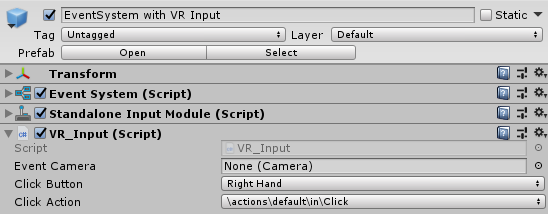
\includegraphics[width=0.5\linewidth]{Bilder/A41_EventSystem}
	\caption{Event System mit VR Input Aufbau in der Szene, eigene Abbildung}
	\label{fig:EventSystem}
\end{figure}
\newline
Der aktuell eingesetzte Pointer in wird sobald das Programm ausgeführt wird als Kind-Objekt des rechten Controllers (Vgl. Abbildung XX) instanziiert. Somit bewegt sich der Pointer mit der rechten Hand bzw. mit dem rechten Controller mit. Zu Beginn wird Standardmäßig der Physics Pointer instanziiert, sobald jedoch ein Objekt angeklickt wird und sich somit das Menü dieses Objektes öffnet, wird auf den Canvas Pointer gewechselt.
\newline
Sowohl der \textbf{Canvas Pointer} als auch der \textbf{Physics Pointer} enthalten die Komponenten Camera, Line Renderer und das zugehörige Skript. Der Physics Pointer enthält zusätzlich die Komponente Physics Raycaster (Vgl. Abbildung XX). Mit Hilfe der Komponente Camera lässt sich bestimmen worauf der aktuelle Pointer zeigt. Diese Komponente wird durch das im späteren Verlauf dieses Kapitels vorgestellte Skript Switch Pointers beim Event System hinterlegt (Vgl. Abbildung XX). Der Line Renderer hat lediglich die Aufgabe eine Linie zu zeichnen, damit der Bediener erkennen kann worauf er klickt. Diese Linie beginnt beim Controller in der rechten Hand des Bedieners und ist standardmäßig drei Unity-Einheiten lang. Falls ein Objekt die Linie schneidet, endet diese an dem Schnittpunkt. 
\newline
Grundsätzlich funktionieren die Klassen VR Physics Pointer und VR Canvas Pointer nach dem gleichen Prinzip. Es wird ausgehend vom Ursprung des Pointers ein Raycast („Strahl“) gesendet und überprüft womit dieser interagiert. Der unterschied ist, dass durch die Klasse VR Physics Pointer ein Raycast gesendet wird, der nur mit Objekten die einen Collidern besitzen interagiert (Physics Raycast). Die Klasse VR Canvas Pointer hingegen sendet mit Hilfe des Event Systems einen Raycast, der nur mit Objekten die Bestandteil einer graphischen Benutzeroberfläche sind interagiert. Daher ist die einzige Anforderung an die Umgebung, dass die Objekte mit denen interagiert werden soll einen Collider besitzen und das die Menüs die bereits in Unity vorhandenen Elemente wie z.B. Knöpfe oder Slider für grafische Benutzeroberflächen nutzen.
\begin{figure}[h]
	\centering
	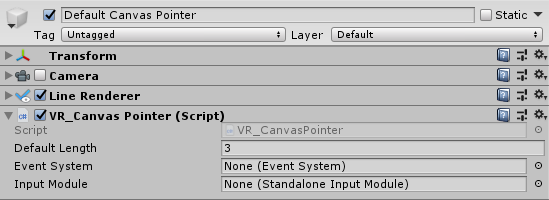
\includegraphics[width=0.5\linewidth]{Bilder/A42_CanvasPointer}
	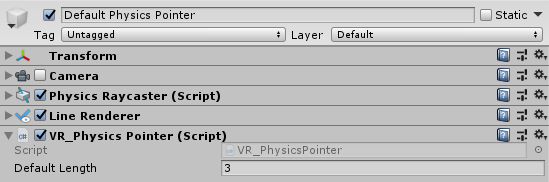
\includegraphics[width=0.5\linewidth]{Bilder/A43_PhysicsPointer}
	\caption{Canvas Pointer und Physics Pointer Aufbau in der Szene, eigene Abbildung}
	\label{fig:Pointer}
\end{figure}
\newline
Der Wechsel zwischen den Pointern wird durch die Klasse \textbf{Switch Pointers} gehandhabt. Diese enthält in öffentlichen Variablen Verweise auf die Objektvorlagen der beiden Pointer (Vgl. Abbildung XX).
\newline
Zu Beginn wird in der Methode Start wie bereits erwähnt ein Physics Pointer instanziiert, dessen Kamera Komponente als Event Camera beim Event System gesetzt wird (Vgl. Abbildung XX). Die Methode Update ruft die Methode HandlePointerSwitch jede Sekunde mehrfach auf. Sobald ein Objekt angeklickt wird und sich sein Menü öffnet, wird der Pointer mit Hilfe der Methode HandlePointerSwitch ausgetauscht und die Event Camera beim Event System aktualisiert. Des Weiteren werden bei dem Canvas Pointer die Referenzen zum Event System und seinem Input Module gesetzt (Vgl. Abbildung XX). Die Beiden Hilfsmethoden SpawnPhysicsPointer und SpawnCanvasPointer kommen zum Einsatz um den entsprechenden Pointer zu instanziieren.
\begin{figure}[h]
	\centering
	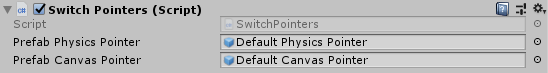
\includegraphics[width=0.5\linewidth]{Bilder/A45_SwitchPointer}
	\caption{Switch Pointers Aufbau in der Szene, eigene Abbildung}
	\label{fig:SwitchPointer}
\end{figure}
\newline
Die letzte Komponente des Grundgerüsts der Interaktionsschnittstelle ist die Klasse \textbf{Object Menu}. Diese Klasse kann zu jedem beliebigen Objekt in der Szene hinzugefügt werden. Die wichtigsten Komponenten dieser Klasse sind die öffentlichen Variablen prefab, thisObject, clickButton und clickAction (Vgl. Abbildung XX). Die Variable prefab enthält den Verweis auf die Objektvorlage des zu öffnenden Menüs und die variable thisObject enthält den Objektverweis auf das Objekt zu dem das Skript gehört. Die Variablen clickButton und clickAction werden lediglich genutzt um die Input-Taste für das Schließen des Menüs zu deklarieren.
\newline
Insgesamt enthält diese Klasse drei Methoden. In der Methode Start werden lediglich ein paar private Hilfsvariablen deklariert und in der Methode Update wird, falls das Objekt angeklickt wird die Methode HandleButtonPress aufgerufen. Diese Methode instanziiert dann eine Instanz des zu öffnenden Menüs. Beim erneuten aufrufen der Methode HandleButtonPress durch das Drücken der entsprechenden Taste am rechten Controller wird das bereits geöffnete Menü wieder geschlossen. Des Weiteren aktualisiert die Methode Update die Position des Menüs mehrmals pro Sekunde, sodass sich das Menü mit der Kopfbewegung des Bediener mitbewegt und stehts gut sichtbar ist.
\begin{figure}[h]
	\centering
	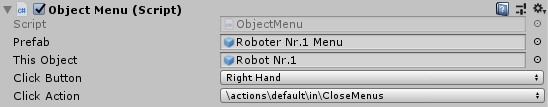
\includegraphics[width=0.5\linewidth]{Bilder/A46_ObjectMenu}
	\caption{Object Menu Aufbau in der Szene, eigene Abbildung}
	\label{fig:ObjectMenu}
\end{figure}		% Umsetzung
%--------------------------------------------------------------------------------------------------	
%--------------------------------------------------------------------------------------------------
\chapter{Validierung des Konzepts}\label{cha:ValidierungDesKonzepts}
In diesem Kapitel wird die Umsetzung des Konzepts mit Hilfe der Unity Engine validiert. Dafür wird zunächst erläutert, wie die in Kapitel \ref{sec:AnforderungenKonzept} gestellten Anforderungen an das Menschmodell und an die Interaktionsschnittstelle erfüllt wurden. Anschließend (TODO...)
%--------------------------------------------------------------------------------------------------
\section{Validierung des Menschmodells}\label{sec:ValidMensch}

\subsection{Anforderung 1: Genauigkeit}
Durch die Möglichkeit, die Bewegungen des Bedieners an bis zu zehn Körperteilen (Beide Füße, beide Knie, Steißbein, beide Hände, beide Ellenbogen und Kopf) zu verfolgen und diese Daten bei der Abbildung auf den virtuellen Menschen zu berücksichtigen, wird die in Kapitel \ref{sec:AnforderungenKonzept} geforderte Genauigkeit erfüllt. Zusätzlich wird die Genauigkeit, durch die Möglichkeit das Menschmodell zu Kalibrieren, also an die Körpergröße des Bedieners anzupassen, verbessert. So könnte man in Zukunft für jeden beliebigen Bediener mit Hilfe des Menschmodells einen virtuellen Klon für die virtuelle Welt schaffen, in dem man die Textur für den in Kapitel \ref{sec:MMModell} angesprochenen Skinned Mesh Renderer anpasst.

\subsection{Anforderung 2: Echtzeit}
Mit Hilfe des Plugins Final IK werden die Bewegungsdaten des Bedieners in nahezu Echtzeit verarbeitet und auf das Menschmodell übertragen. Es sind keine sichtbaren Verzögerungen zu erkennen, die die Nützlichkeit des Menschmodells einschränken würden oder sogar eine potenzielle Gefahrenquelle darstellen könnten. Aufgrund dessen wird die in Kapitel \ref{sec:AnforderungenKonzept} gestellte Anforderung an die Echtzeit ebenfalls erfüllt.

\subsection{Anforderung 3: Interoperabilität}
Das Menschmodell wurde umgebungsunabhängig implementiert, ist also von keinen anderen Komponenten der virtuellen Umgebung abhängig. Folglich kann das Menschmodell in jeder beliebigen virtuellen Umgebung, wie Beispielsweise virtuell begehbare Produktionsanlagen, eingesetzt werden und erfüllt somit die in Kapitel \ref{sec:AnforderungenKonzept} gestellte Anforderung an die Interoperabilität.

\subsection{Anforderung 4: Modularität}
Wie in Abbildung \ref{fig:UnityOverview} zu erkennen ist, ist das Menschmodell modular aufgebaut und erlaubt einfache Anpassungen und Erweiterungen in der Zukunft. Insgesamt besteht das Menschmodell (ohne die Interaktionsschnittstelle) aus den vier Komponenten Kamera, Modell, Skripte und Verfolgungsziele, welche selber nochmal aus einigen Komponenten bestehen. Aufgrund dessen wird die in Kapitel \ref{sec:AnforderungenKonzept} geforderte Modularität gewährleistet.

%--------------------------------------------------------------------------------------------------
\section{Validierung der Interaktionsschnittstelle}\label{sec:ValidInteraktion}

\subsection{Anforderung 1: Bidirektionalität}
Der Informationsaustausch zwischen Mensch und Maschine findet bidirektional statt, da der Mensch durch den Pointer die Möglichkeit erhält über graphische Benutzeroberflächen mit der Maschine zu interagieren. In anderen Worten stellt der Pointer das Input-Medium des Menschen dar. Gleichzeitig ermöglichen die graphischen Benutzeroberflächen die Darstellung von Feedback der Produktionsanlagen. So könnten Beispielsweise Produktionsraten, Stromverbrauch oder sonstige produktionstechnisch relevante Parameter angezeigt werden. Aufgrund dessen wird die in Kapitel \ref{sec:AnforderungenKonzept} geforderte Anforderung der Bidirektionalität erfüllt.

\subsection{Anforderung 2: Genauigkeit}
Mit Hilfe des Pointers, der durch das Bewegen der rechten Hand gesteuert wird, wird ein sehr präzises und vor allem intuitives interagieren mit der Umgebung ermöglicht. Aufgrund dessen wird die in Kapitel \ref{sec:AnforderungenKonzept} geforderte Genauigkeit bei der Interaktion mit der Umgebung gewährleistet.

\subsection{Anforderung 3: Echtzeit}
Durch die Verarbeitung der Bewegungsdaten in Echtzeit wird nicht nur die nahezu verzögerungslose Abbildung des Menschmodells, sondern auch eine nahezu verzögerungslose Interaktion mit der Umgebung ermöglicht. Dies ermöglicht den Bedienern schnell auf Veränderungen in der virtuellen Umgebung zu reagieren und spontane Anpassungen zu tätigen. Aufgrund dessen wird die in Kapitel \ref{sec:AnforderungenKonzept} gestellte Anforderung an die Echtzeit ebenfalls erfüllt.

\subsection{Anforderung 4: Interoperabilität}
Die Interaktionsschnittstelle ist, bis auf wenige Skripte und dem Interaktionssystem, nicht von der Umgebung abhängig. Daher ist es ausreichend, die eben angesprochenen Komponenten irgendwo in der Szene zu hinterlegen (Vgl. Abbildung \ref{fig:UnityOverview}). Um eine Interaktion mit beliebigen Objekten in der Szene zu ermöglichen, müssen diese lediglich mit dem Object Menu Skript und einem Collider erweitert werden. Des Weiteren müssen ihre Menüs mit Hilfe der bereits in Unity vorhanden Komponenten für graphische Benutzeroberflächen implementiert sein. Folglich wird die in Kapitel \ref{sec:AnforderungenKonzept} geforderte Interoperabilität gewährleistet, da sich die beschrieben Funktionalität auf beliebige Objekte übertragen lässt, solange die entsprechenden Rahmenbedingungen eingehalten werden.

\subsection{Anforderung 5: Modularität}
Sowohl das Menschmodell, als auch die Interaktionsschnittstelle sind Modular aufgebaut und bestehe aus austauschbaren Komponenten. Es ist beispielsweise möglich, die Interaktionsschnittstelle für andere VR Hardware einsatzfähig zu machen. Dafür müssen lediglich die entsprechenden Input Schnittstellen der VR Hardware in einigen Skripten angepasst werden. Des Weiteren wurden das Menschmodell und die Interaktionsschnittstelle getrennt voneinander entwickelt, um die Unabhängigkeit und somit die in Kapitel \ref{sec:AnforderungenKonzept} geforderte Modularität zu gewährleisten.

%--------------------------------------------------------------------------------------------------
\section{Vorgehen beim hinzufügen von Objekten in der Szene}\label{sec:ValidVorgehen}
--> Auch das mit falko hier			% Validierung des Konzepts
%--------------------------------------------------------------------------------------------------	
%--------------------------------------------------------------------------------------------------
\chapter{Ausblick und Zusammenfassung}\label{cha:AusblickUndFazit}

Einige der in Kapitel \ref{sec:PotentialeIndustrie4.0} dieser Arbeit vorgestellten Potenziale von Industrie 4.0, konnten durch das bei dieser Arbeit entstandene und in Kapitel \ref{cha:Umsetzung} vorgestellte Anwendungsbeispiel einer virtuellen Umgebung, in der mittels eines Menschmodells und einer Interaktionsschnittstelle mit beliebigen Objekten interagiert werden kann, verdeutlicht werden. Dabei sind die Potenziale zehn („Simulation und Überwachung der Produktion") und elf („Chancen für IT-Unternehmen") besonders hervorzuheben.
\newline
Mit Hilfe der in Kapitel \ref{sec:PhysischZumKlon} vorgestellten Vorgehensweise für die Schaffung eines virtuellen Klons einer Produktionsanlagen und mit Hilfe des in Kapitel \ref{cha:Umsetzung} vorgestellten Menschmodells inklusive der Interaktionsschnittstelle, eröffnet sich die Möglichkeit, in Zukunft Produktionsstätten über einen virtuellen Zwilling zu begehen, mit einzelnen Produktionsanlagen zu interagieren und diese somit zu steuern. Aufgrund dessen könnte in Zukunft die Wettbewerbsfähigkeit des Hochlohnstandorts Deutschland verbessert werden, da die über einen virtuellen Zwilling gesteuerten Produktionsanlagen an jedem beliebigen Standort auf der Welt stehen könnten.
\newline
Angetrieben durch den damit verbundenen technologischen Entwicklungsaufwand, eröffnen sich vor allem für IT-Unternehmen Chancen am Wandel zu Industrie 4.0 zu profitieren, da der Wandel zu Industrie 4.0 ein von vielen Herausforderungen geprägter und interdisziplinärer Prozess ist und die daher Ausmaße des klassischen Maschinenbaus übersteigt. Dies wird unter anderem durch die in Kapitel \ref{sec:HerausforderungenUmsetzung} vorgestellten Herausforderungen verdeutlicht. Insbesondere fehlt der zweite Schritt der in Kapitel \ref{sec:MMInteraktion} erläuterten Mensch-Maschine-Interaktion, um die in Unity erschaffene, begehbare und interagierbare virtuelle Umgebung mit den realen Produktionsanlagen zu verbinden. Diese Aufgabe war zum Zeitpunkt des Schreibens dieser Arbeit ebenfalls das Thema einer Bachelorarbeit eines Informatik Studenten am Fachgebiet DiK (Datenverarbeitung in der Konstruktion) der Technischen Universität Darmstadt.

%--------------------------------------------------------------------------------------------------
\section{Ausblick}\label{sec:Ausblick}
Es bleibt die Frage, wie Industrie 4.0 in Zukunft aussehen wird. Durch die gewonnenen Erkenntnisse beim Recherchieren und Verfassen dieser Arbeit, lässt sich eindeutig sagen, dass es keine allgemeine Lösung gibt und geben kann. Wie bereits in Kapitel \ref{sec:LeitfadenUmsetung} angedeutet, stehen Unternehmen vor der schwierigen Herausforderungen, die Industrie 4.0 Potenziale in ihrem Unternehmen zu erkennen und unter Berücksichtigung der in Kapitel \ref{sec:HerausforderungenUmsetzung} vorgestellten Herausforderungen umzusetzen. Diese Potenziale können im Zeitalter des Internets der Dinge und Dienstleistungen nicht nur im optimieren der Produktionsprozesse oder der Ressourceneffizienz, sondern auch in der Gestaltung neuer Dienstleistungen (Smart Services) und vielen weiteren Bereichen liegen (Vgl. Kapitel \ref{sec:PotentialeIndustrie4.0}). 
Einziger Anhaltspunkt für Unternehmen sind die Industrie 4.0 Leitfäden aus Kapitel \ref{sec:LeitfadenUmsetung}. Dabei ist anzumerken, dass diese mit Hilfe von Werkzeugkästen, Handlungsfeldern, Rahmenbedingungen oder ähnlichem die Unternehmen lediglich dabei Unterstützen sollen, einen eigenen Weg für die Umsetzung von Industrie 4.0 zu finden.
\newline\newline
Des Weiteren stellt sich die Frage, inwiefern Virtual Reality (virtuelle Realität) beim Wandel zu Industrie 4.0 eine Rolle spielt. Wie bereits in Kapitel \ref{sec:VRGeschichte} dargestellt, befinden wir uns am Anfang einer neuen Phase der Virtual Reality. Dabei findet Virtual Reality neue Einsatzmöglichkeiten in verschiedensten Lebensbereichen, von Bildung bis hin zu Industrie. Als Teil der Disziplin Visual Computing, welche als eine Schlüsselkomponente beim Wandel zu Industrie 4.0 angesehen wird \cite[S.1]{17}, eröffnen sich durch den Einsatz von Virtual Reality viele Potenziale für neue Wertschöpfungsprozesse. Dazu gehört Beispielsweise, die bereits mehrfach erwähnte Möglichkeit einer standortunabhängigen Steuerung von Produktionsanlagen.

%--------------------------------------------------------------------------------------------------3
\section{Zusammenfassung der wichtigsten Ergebnisse}\label{sec:ZusammenfassungErgebnisse}
Zunächst wurde in Kapitel \ref{cha:StandDerTechnik} dieser Arbeit der aktuelle Stand der Technik, insbesondere im Hinblick auf Industrie 4.0, der Ausgangslage der industriellen Fertigung und der Geschichte von Virtual Reality aufgearbeitet
Daraufhin wurde in Kapitel \ref{cha:AufbauDesKonzepts}, basierend auf dem Prozess von der physischen Produktionsanlage bis hin zu ihrem virtuellen Klon, der Mensch-Maschine Interaktion im Kontext dieser Arbeit und dem FMI Standard, ein Konzept geschaffen und Anforderungen definiert.
Anschließend wurde in Kapitel \ref{cha:Umsetzung}, nach einer Einführung in die verwendete Hardware und Software, die Umsetzung des Menschmodells und der Interaktionsschnittstelle mit Hilfe der Unity Engine erläutert. 
Schließlich wurde in Kapitel \ref{cha:ValidierungDesKonzepts} die Vorgehensweise beim Einbinden des entstandenen Menschmodells in ein neues Projekt und die Vorgehensweise beim Einfügen neuer Objekte in der Umgebung erläutert, bevor die zuvor gestellten Anforderungen an das Menschmodell und die Interaktionsschnittstelle validiert wurden.
\newline\newline
Die zentrale Aufgabe dieser Arbeit war es, ein Menschmodell zu schaffen, welches die Bewegungen des Bedieners in der virtuellen Welt verzögerungsfrei Abbildet und dem Bediener ermöglicht mit der virtuellen Umgebung zu interagieren. Dabei mussten insbesondere die letzten zwei, der in Kapitel \ref{sec:AnforderungenKonzept} erläuterten Anforderungen Genauigkeit, Echtzeit, Interoperabilität und Modularität gewährleistet werden, um zukünftige Anpassungen am Menschmodell und das problemlose Zusammenfügen des eigentlichen Menschmodells mit der separat entwickelten Interaktionsschnittstelle zu ermöglichen.
\newline
Wie bereits erwähnt, wurde die Interaktionsschnittstelle unabhängig vom Menschmodell, mit Fokus auf die in Kapitel \ref{sec:AnforderungenKonzept} gestellten Anforderungen Bidirektionalität, Genauigkeit, Echtzeit, Interoperabilität und Modularität, entwickelt. Sowohl die Anforderungen an das Menschmodell, als auch die Anforderungen an die Interaktionsschnittstelle konnten durch die Art und Weise der Umsetzung, wie bereits in Kapitel \ref{sec:ValidMensch} und \ref{sec:ValidInteraktion} erläutert, gewährleistet werden.
\newline
Wegweisend waren dabei die in Kapitel \ref{sec:DasFMU} gewonnenen Kenntnisse über das Functional-Mockup Interface, da das entstandene Menschmodell, ähnlich wie eine FMU bei einer Co-Simulation, nur ein Bestandteil einer größeren Anwendung ist. Die Vollendung der Mensch-Maschine Schnittstelle, also das Verbinden der virtuellen Umgebung in Unity mit echten Produktionsanlagen, durch das Zusammenfügen mit der bereits angesprochenen Arbeit eines anderen Studenten am DiK, sollte dank der Einhaltung der Anforderungen an die Modularität und Interoperabilität, mit geringen Aufwand möglich sein.
\newline\newline
Aufgrund des entstandenen Anwendungsbeispiels, vor allem in Kombination mit dem zweiten Schritt der Mensch-Maschine Interaktion, offenbart sich die Möglichkeit einer maßgeblichen Wandlung der Industrie, bei der insbesondere die Standortunabhängigkeit von Unternehmen gestärkt wird. Dadurch könnte in Zukunft das zentrale Leitmotiv von Firmen aus dem Produktionsbereich "Designed by us, produced anywhere" \cite{34} lauten.
%1 \cite{1} 2 \cite{2} 3 \cite{3} 4 \cite{4} 5 \cite{5} 6 \cite{6} 7 \cite{7} 8 \cite{8}
%9 \cite{9} 10 \cite{10} 11 \cite{11} 12 \cite{12} 13 \cite{13} 14 \cite{14} 15 \cite{15}
%16 \cite{16} 17 \cite{17} %18 \cite{18} 
%19 \cite{19} 20 \cite{20} 21 \cite{21} 22 \cite{22}
%23 \cite{23} 24 \cite{24} 25 \cite{25} 26 \cite{26} 27 \cite{27} 28 \cite{28} 29 \cite{29}
%30 \cite{30} 31 \cite{31} 32 \cite{32} 33 \cite{33} 34 \cite{34} A1 \cite{A1} A2 \cite{A2} 
%A14 \cite{A14} A15 \cite{A15} A16 \cite{A16} A18 \cite{A18} A26 \cite{A26} A27 \cite{A27} 
%A28 \cite{A28} A29 \cite{A29}
%--------------------------------------------------------------------------------------------------					% Ausblick und Fazit
%--------------------------------------------------------------------------------------------------	
\cleardoublepage											% Cleardoublepage
\pagenumbering{roman}\setcounter{page}{6}					% Römische Nummerierung fortsetzen
\phantomsection												% Phantomsection
\addcontentsline{toc}{chapter}{Literaturverzeichnis}		% Verlinkung im Inhaltsverzeichnis
\printbibliography											% Literatur Verzeichnis
\cleardoublepage											% Cleardoublepage
%--------------------------------------------------------------------------------------------------	
\phantomsection												% Phantomsection
\addcontentsline{toc}{chapter}{Anhang}						% Verlinkung im Inhaltsverzeichnis
\chapter*{Anhang} \label{cha:Anhang}

Zusätzlich zu dieser schriftlichen Ausarbeitung und der Implementierung mit Hilfe der Unity Engine, habe ich eine kurze Erklärung des Projekts gefilmt. Diese Video-Datei wird gemeinsam mit der schriftlichen Ausarbeitung und der Implementierung abgegeben. Es ist anzumerken, dass für ein besseres Verständnis des Videos, vorher die Kapitel \ref{cha:Umsetzung} und Kapitel \ref{cha:ValidierungDesKonzepts} dieser Arbeit sorgfältig durchgelesen werden sollten. Das Video ist insgesamt ca. 28 Minuten lang und besteht aus den Folgenden fünf Abschnitten:
\begin{enumerate}
	\item \textbf{Einleitung} \\
	Zunächst gibt es eine kurze Einleitung und Begrüßung.
	\item \textbf{Programme Starten} \\
	Daraufhin wird erläutert, welche Programme gestartet werden müssen.
	\item \textbf{VR-Hardware-Anzug anziehen} \\
	Anschließend gibt es eine Erklärung bezüglich der VR-Hardware.
	\item \textbf{Live-Demo} \\
	Als nächstes gibt es eine Live-Demo, in der sämtliche Funktionalitäten vorgestellt werden.
	\item \textbf{Erklärung des Projekts} \\
	Schließlich gibt es eine ausführliche Erklärung über den Aufbau und die Funktionsweise des Projekts (Skripte, Szene und Ordnerstruktur).
\end{enumerate}
							% Anhang
\cleardoublepage											% Cleardoublepage
%--------------------------------------------------------------------------------------------------	
\end{document}												% Ende des Dokuments